\documentclass[smallextended]{svjour3}

\usepackage{cite}
\usepackage{amsmath,amssymb,amsfonts}
\usepackage{algorithmic}
\usepackage{graphicx}
\usepackage{textcomp}
\usepackage{xcolor}
\usepackage[framemethod=TikZ]{mdframed}
\usepackage{multirow}
\usepackage{array}
\usepackage{lipsum}
% \usepackage{subfigure}
\usepackage{caption}
\usepackage{subcaption}
\usepackage{hyperref}
\usepackage{longtable}


\newcommand{\specialcell}[2][c]{%
  \begin{tabular}[#1]{@{}c@{}}#2\end{tabular}}

\usepackage{xspace}
\newcommand{\instance}{{\em CTO}\xspace}
\newcommand{\inconsistent}{{\em IoPV}\xspace}

\newcommand{\ian}[1]{\textcolor{red}{{\it [Ian says: #1]}}}
\newcommand{\bram}[1]{\textcolor{orange}{{\it [Bram says: #1]}}}
\newcommand{\heng}[1]{\textcolor{blue}{{\it [Heng says: #1]}}}
\newcommand{\med}[1]{\textcolor{cyan}{{\it [Mohammed says: #1]}}}
\newcommand{\jinfu}[1]{\textcolor{purple}{{\it [Jinfu says: #1]}}}
% \newcommand{\heng}[1]{\textcolor{green}{{\it [Heng says: #1]}}}

\def\BibTeX{{\rm B\kern-.05em{\sc i\kern-.025em b}\kern-.08em
    T\kern-.1667em\lower.7ex\hbox{E}\kern-.125emX}}
    
    
\usepackage[most]{tcolorbox}

\hypersetup{
  colorlinks,
  citecolor=blue,
  linkcolor=red,
  urlcolor=purple}

\definecolor{custom-gray}{cmyk}{0, 0, 0, 0.7, 1.00}
\newtcbtheorem[no counter]{Summary}{\hskip-0.97em}{enhanced,drop shadow={black!50!white},
  coltitle=white,
  top=0.1in,
  attach boxed title to top left=
  {xshift=1em,yshift=-\tcboxedtitleheight/2},
  boxed title style={size=small,colback=custom-gray}
}{summary}

\newcommand{\PQI}{Are \inconsistent issues common in the studied systems? }
\newcommand{\PQII}{How difficult is it to manually identify \inconsistent issues?}

\newcommand{\RQI}{What is the impact of configuration on performance regression?}
\newcommand{\RQII}{Can we accurately learn \inconsistent issues in the studied systems? }
\newcommand{\RQIII}{What are the most important metrics for predicting \inconsistent issues? }


\definecolor{dkgreen}{rgb}{0,0.6,0}
\definecolor{gray}{rgb}{0.5,0.5,0.5}
\definecolor{mauve}{rgb}{0.58,0,0.82}
\lstset{frame=tb,
	language=Java,
	aboveskip=3mm,
	belowskip=3mm,
	showstringspaces=false,
	columns=flexible,
	basicstyle={\small\ttfamily},
	numbers=none,
	%numberstyle=\tiny\color{gray},
	%keywordstyle=\color{blue},
	%commentstyle=\color{dkgreen},
	%stringstyle=\color{mauve},
	breaklines=true,
	breakatwhitespace=true,
	tabsize=3
}


\newcommand{\specialcell}[2][c]{%
	\begin{tabular}[#1]{@{}c@{}}#2\end{tabular}}

\usepackage{multirow}
\usepackage{graphicx}
\usepackage[flushleft]{threeparttable}
\usepackage{flushend}

\usepackage[round,sort]{natbib}

\usepackage{array}
\newcolumntype{L}[1]{>{\raggedright\let\newline\\\arraybackslash\hspace{0pt}}m{#1}}
\newcolumntype{C}[1]{>{\centering\let\newline\\\arraybackslash\hspace{0pt}}m{#1}}
\newcolumntype{R}[1]{>{\raggedleft\let\newline\\\arraybackslash\hspace{0pt}}m{#1}}
\begin{document}

\title{Using Black-Box Performance Models to Detect Performance Regressions under Varying Workloads: An Empirical Study}

%\titlerunning{shorter title}
\author{Lizhi Liao \and
	    Jinfu Chen \and
	    Heng Li \and
	    Yi Zeng \and
	    Weiyi Shang \and
	    Jianmei Guo \and
	    Catalin Sporea \and 
	    Andrei Toma \and
	    Sarah Sajedi
}

\institute{Lizhi Liao, Jinfu Chen, Yi Zeng, Weiyi Shang\at
	Department of Computer Science and Software Engineering\\
	Concordia University\\
	Montreal, Quebec, Canada\\
	\email{\{l\_lizhi, fu\_chen, ze\_yi, shang\}@encs.concordia.ca} \\\\
	Heng Li\at
	Software Analysis and Intelligence Lab (SAIL)\\
	Queen’s University\\
	Kingston, Ontario, Canada\\
	\email{hengli@cs.queensu.ca} \\\\
	Jianmei Guo \at
	Alibaba Group\\
	Hangzhou, Zhejiang, China\\
	\email{jianmei.gjm@alibaba-inc.com} \\\\
	Catalin Sporea, Andrei Toma,Sarah Sajedi \at
	ERA Environmental Management Solutions\\
	Montreal, Quebec, Canada\\
	\email{\{steve.sporea, andrei.toma, sarah.sajedi\}@era-ehs.com}
}

\date{Received: date / Accepted: date}

% make the title area
\maketitle

\begin{abstract}
    Performance regressions of large-scale software systems
    often lead to both financial and reputational losses.
    In order to detect performance regressions, performance tests are typically conducted in an in-house (non-production) environment using test suites with predefined workloads. 
    Then, performance analysis is performed to check whether a software version has a performance regression against an earlier version. 
    However, the real workloads in the field are constantly changing, making it unrealistic to resemble the field workloads in predefined test suites. 
    More importantly, performance testing is usually very expensive as it requires extensive resources and lasts for an extended period. 
    In this work,
    we leverage black-box machine learning models to automatically detect performance regressions in the field operations of large-scale software systems.
    Practitioners can leverage our approaches to complement or replace resource-demanding performance tests that may not even be realistic in a fast-paced environment.
    Our approaches use black-box models to capture the relationship between the performance of a software system (e.g., CPU usage) under varying workloads and the runtime activities that are recorded in the readily-available logs. 
    Then, our approaches compare the black-box models derived from the current software version with an earlier version to detect performance regressions between these two versions.
    We conducted a case study on two open source systems 
    and one large-scale industry system. 
    Our results show that such black-box models can effectively and timely detect real performance regressions and injected ones under varying workloads that are unseen when training these models.
    Our approaches have been adopted in practice to detect performance regressions of a large-scale industry system on a daily basis. 
  	
\end{abstract}

\keywords{Performance regression \and Black-box performance models \and Field workloads \and Performance engineering}

\section{Introduction} \label{sec:intro}

Many large-scale software systems (e.g., Amazon, Google, Facebook) provide services to millions or even billions of users every day.
Performance regressions in such systems usually lead to both reputational and monetary losses. 
For example, a recent incident of performance regressions at Salesforce\footnote{https://www.salesforce.com} affected eight data centers, resulting in a negative impact (i.e., slowdown and failures of the provided services) on the experience of clients across many organizations ~\citep{SaleForcePerfDegradation2019}.
It is reported that 59\% of Fortune 500 companies experience at least 1.6 hours of downtime per week~\citep{SyncsortWhitePaper2018}, while most of the field failures are due to performance issues rather than feature issues~\citep{DBLP:journals/tse/WeyukerV00}.
To avoid such performance-related problems, practitioners perform in-house performance testing to detect performance regressions of large-scale software systems~\citep{DBLP:journals/tse/JiangH15}.

For in-house performance testing, load generators (e.g., JMeter\footnote{https://jmeter.apache.org}) are used to mimic thousands or millions of users (i.e., the \emph{workload}) accessing the system under test (SUT) at the same time.
Performance data (e.g., CPU usage) is recorded during the performance testing for later performance analysis.
To determine whether a performance regression exists, the performance data of the current software version is compared to the performance data from running an earlier version on the same workload, using various analysis techniques~\citep{DBLP:conf/icst/GaoJBL16} (e.g., control charts~\citep{DBLP:conf/wosp/NguyenAJHNF12}).
However, such in-house performance testing suffers from two important challenges.
First, the real workloads in the field are constantly changing and difficult to predict~\citep{DBLP:conf/wosp/SyerJNHNF14}, making it unrealistic to test such dynamic workloads in a predefined manner.
Second, performance testing is usually very expensive as it requires extensive resources (e.g., computing power) and lasts for a long time (e.g., hours or even weeks).
For software systems that follow fast release cycles (e.g., Facebook is released every few hours), performance testing becomes particularly difficult.


In this work, we aim at directly detecting performance regressions in the field operations of large-scale software systems.
Such an automated detection can complement or even replace typical in-house performance testing when testing resources are limited (e.g., in an agile environment) and/or filed workloads are challenging to be reproduced in testing.
In particular, we leverage sparsely-sampled performance metrics and readily-available execution logs from the field to detect performance regressions, which only adds negligible performance overhead to SUT.
Inspired by prior research~\citep{Yao:2018:LSL:3184407.3184416,DBLP:conf/issre/FarshchiSWG15}, we use machine learning techniques (i.e., black-box performance models) to capture the relationship between the runtime activities that are recorded in the readily-available logs of a software system and its performance metrics under such activities. 
We use the black-box model that describes the current version of a software system and the black-box model that describes an earlier version of the same software system, to determine the existence of performance regressions between these two versions.

We conducted an empirical study on two open source systems (i.e., OpenMRS and Apache James) and one large-scale industrial system. 
In particular, our study aims to answer two research questions (RQs):

\begin{description}
\item[\textbf{RQ1:}] \textit{How well can we model system performance under varying workloads?} \\ 
In order to capture the performance of a system under varying workloads, we built six machine learning models (including three traditional models and three deep neural networks).
We found that simple traditional models can effectively capture the relationship between the performance of a system and its dynamic activities that are recorded in logs. 
In addition, such models can equivalently capture the performance of a system under new workloads that are unseen when building the models.

\item[\textbf{RQ2:}] \textit{Can our approaches detect performance regressions under varying workloads?} \\ 
Our black-box model-based approaches can effectively detect both the real performance regressions and injected ones under varying workloads (i.e., when the workloads are unseen when training the black-box models).
Besides, our approaches can detect performance regressions with the data from a short period of operations, enabling early detection of performance regressions in the field.

\end{description}

Our work makes the following key contributions:
\begin{itemize} 
    \item Our study demonstrates the effectiveness of using black-box machine learning models to model the performance of a system when the workloads are evolving (i.e., the model trained on a previous workload can capture the system performance under new unseen workloads). %against its dynamic activities in field operations.
    %\item Our study demonstrates the effectiveness of leveraging operational data (e.g., logs and performance metrics) from the field and black-box machine learning models to detect performance regressions in the field.
    \item Our experiments on one large-scale industry system and two open source systems show that we can use black-box machine learning models to detect performance regressions in the field where workloads are constantly evolving (i.e., two releases of the same system are never running the same workloads).
    \item Our approaches can complement or even replace traditional in-house performance testing when testing resources are limited.
    \item We shared the challenges and the lessons that we learned from the successful adoption of our approaches in the industry, which can provide insights for researchers and practitioners who are interested in detecting performance regressions in the field.
\end{itemize}

The remainder of the paper is organized as follows. 
Section~\ref{sec:background} introduces the background of black-box performance modeling.
Section~\ref{sec:approach} outlines our approaches for detecting performance regressions in the field.
Section~\ref{sec:casestudysetup} and Section~\ref{sec:casestudyresults} present the setup and the results of our case study on three subject systems, respectively.
The challenges and the lessons that we learned from the successful adoption of our approaches are discussed in Section~\ref{sec:challenges}.
Section~\ref{sec:threats} and Section~\ref{sec:relatedwork} discuss the threats to the validity of our findings and the related work, respectively.
Finally, Section~\ref{sec:conclusions} concludes the paper.




\section{Background}
\label{sec:back}


%\subsection{Configuration}

Software configuration is a mechanism used to customize the behaviour of a software system without changing the source code. The configuration \textbf{options} are often stored in configuration files as a set of key - value pairs, where the key represents an option's name and the \textbf{value} represents a default or user-chosen value for that option. We define a \textbf{configuration} as one particular assignment of a value to all existing options. Table~\ref{tab:terms} lists the definition of these terms. For example, \emph{A=1} and \emph{B=2} is one possible configuration for a software system with the two integer options \emph{A} and \emph{B}. Configuration options enable users to adapt the execution of their software systems by simply modifying the values of certain configuration options, without re-compilation. For example, a user can change the directory that stores the cache for \emph{Cassandra} by changing the value of the \textit{saved\_caches\_directory} configuration option.% Such configuration can be changed at run-time without changing or recompiling the source code of the whole software system.

\begin{table}[t]
    \centering
    \footnotesize
    \tabcolsep=0.05cm
    \caption{Our definition of configuration, option, and value}
    \begin{tabular}{|p{1.1cm}|p{5.8cm}|l|}
        \hline
        Term & Definition & Example \\
        \hline
        \textbf{Option}  & A typed, configurable item that allows users to set different values. & $A$ \\ \hline
        \textbf{Value} & A specific assignment of a value for an option. & $A = 1$ \\ \hline
        \textbf{Configu-ration} & An assignment of values to all options by a user. & $A = 1; B = 2$ \\ 
        \hline
    \end{tabular}
    \label{tab:terms}
\end{table}


Although configuration introduces large flexibility for users, considering all the possible configurations during testing is impossible. A software system with \jinfu{10} boolean configuration options requires testing $2{^1^0}$ configurations. In fact, configuration problems are among the dominant %\bram{exaggeration (since one of citations is ours)?} 
problems in software engineering~\cite{tse,RN2897}.

In particular, a software system can suffer from what we refer to as \textbf{Inconsistent Option Performance Variation} (a.k.a, \inconsistent). This occurs when, for a given commit \emph{C}, the performance of a subset of an option's values evolved differently relative to their performance in the commit prior to \emph{C}. Considering the example in Figure \ref{fig:description}, when comparing the raw performance of the two option values \emph{V1} and \emph{V2} (Figure~\ref{fig:description-a}), we observe that \emph{V1} shows a better performance than \emph{V2}. However, that might not be problematic as \emph{V2} might just enable an extra feature, such as logging a transaction. In fact, Figure~\ref{fig:description-c} shows that even if \emph{V2} does not show any significant performance variation from the prior commit, \emph{V1} suffers from a performance regression.  
Similarly, in Figure~\ref{fig:description-d} the performance of \emph{V2} is improved compared to the prior commit, while that improvement does not manifest under option value \emph{V1}. The \inconsistent may directly affect the user experience, increase the resources cost of the system and lead to reputational repercussions. %\bram{here (and also in intro) we need to argue that this is a more important problem than the first one, but right now this is not entirely convincing/concrete enough} %That indicates the first type of \inconsistent, which consists of an inconsistent improvement across different values of the same option. 
A performance variation is calculated as the difference between the performance variation of each option's value after and before each commit, which is illustrated in Figure~\ref{fig:description} by ``$a - b$''.


%%% Local Variables:
%%% mode: latex
%%% TeX-master: "../main"
%%% End:


\section{Approaches} \label{sec:approach}


In this section, we present our three approaches that automatically detect performance regression in a new version of a software system based on the logs and performance metrics that are collected under varying workloads. Our approach contains three main steps: 1) preparing data, 2) building black-box performance models, and 3) detecting performance regressions. The three approaches share the first two steps, while being different in the third step. The overview of our studied approaches is shown in Figure~\ref{fig:overview}.

\subsection{Preparing data}
We aim to identify whether there is performance regression in the new version of the system based on modeling the relationship between the performance metrics, e.g., CPU usage, that are recorded during system execution and the corresponding logs that are generated during system execution.

\subsubsection{Splitting data into time periods}
We would like to establish the relationship between the execution of the system and the performance of the system during run time. Since both performance metrics and logs are generated during system runtime and are not synchronized, i.e., there is no corresponding record of performance metric for each line of logs, we would first align the logs and records of performance metrics by splitting them into time periods. For example, one may split a  two-hours dataset into 120 time periods where each time period is one minute in the data. Each log line and each record of performance metric are allocated into their corresponding time period. Then, we consider the aggregation (e.g., taking the average) of the records of performance metrics as the value of the performance metric of the time period, similar as prior research~\citep{Foo:2010:MPR:1848650.1849222}. 

\subsubsection{Extracting log metrics}

We collect logs that are readily generated during the execution of software systems. Such logs represent the execution of the system as workload during a period of time. We then calculate log metrics based on those logs. In particular, we parse the collected logs into events and their corresponding time stamps. For example, a line of web log "\emph{[2019-09-27 22:43:13] GET /openmrs/ws/rest/v1/person/ HTTP/1.1 200}" will be parsed into the corresponding web request or url "\emph{GET /openmrs/ws/rest/v1/person/}" and time stamp "2019-09-27 22:43". Afterwards, each value of a log metric is the number of times that each log event executes during the period. For example, if the log event "\emph{GET /openmrs/ws/rest/v1/person/}" is executed 10 times during a 30-second time period, the corresponding log metric for "\emph{GET /openmrs/ws/rest/v1/person/}"’s value is 10 for that period. 


\begin{figure*}[tbh]
  \centering
  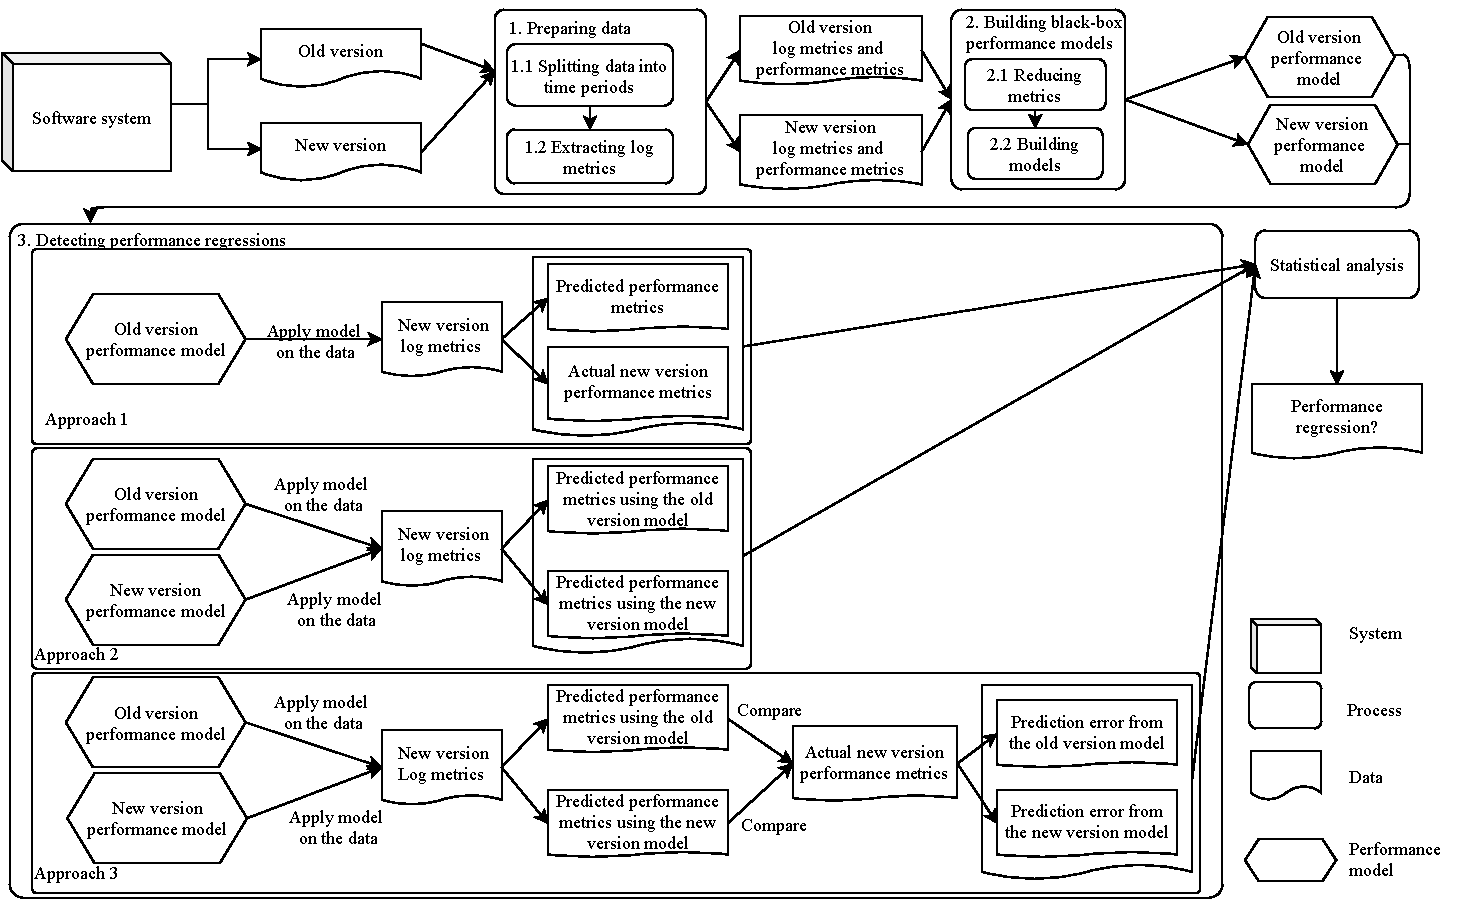
\includegraphics[width=\textwidth]{overview.pdf}
  \caption{An overview of our studied approaches of detecting performance regressions.}
  \label{fig:overview}
\end{figure*}



\subsection{Building black-box performance models}
\label{sec:buildmodel}
In this step, we build black-box models based on the log metrics and performance metrics that are collected and calculated from the data that is generated during system runtime under varied workloads. 

\subsubsection{Reducing metrics}
The frequency of some log events (e.g., periodical events) may not change over time.
The constant appearance of such events may not provide information about the changes of system workloads.
Therefore, after we calculate the log metrics of each log event, we reduce log metrics by removing redundant log metrics or log metrics with constant values in both previous and current versions. We first remove log metrics that have zero variance in both versions of the performance tests. 

Different log events may always appear at the same time, e.g., user logging in and checking user's privilege, and provide repetitive information for the workloads. To avoid the bias from such repetitive information, we then perform correlation analysis and redundancy analysis on each log metrics. We use Pearson's correlation coefficient~\citep{benesty2009pearson} among all log metrics. If a pair of log metrics has a correlation higher than $0.7$, we remove the metric from the two metrics. We repeat such process until there exists no correlation higher than $0.7$. The redundancy analysis would consider a log metrics redundant if it can be predicted from a combination of other log metrics. We use each log metrics as a dependent variable and use the rest of log metrics as independent variables to build a regression model. We calculate the $R^2$ of each model. If the $R^2$ is larger than a threshold (e.g., 0.9), the current dependent variable (i.e., the log metrics) is considered redundant. We then remove the log metric with the highest $R^2$ and repeat the process until no log metrics can be predicted with $R^2$ higher than the threshold. 

We only apply this step when using traditional statistical models or machine learning models (like linear regression or random forest), while if a deep neural network (like convolutional neural network or recurrent neural network) is adopted to build the black-box performance models, we skip this step.


\subsubsection{Building models}
We build models that capture the relationship between a certain workload that is represented by the logs and the system performance. In particular, the independent variables are the log metrics from the last step and the dependent variable is the target performance metric (e.g., CPU usage). One may choose different types of statistical, machine learning or deep learning models, as our approach is agnostic to the choice of models. However, the results of using different types of models may vary (cf. RQ1). 


\subsection{Detecting performance regressions} \label{sec:comparions-approaches}

The goal of building the performance models is to detect performance regressions. Therefore, in this step, we use the black-box performance models that are built from an old version of the system to predict the expected system performance of a new version. Then, we use statistical analysis to determine whether there exists performance deviance based on prediction errors of the models.

Intuitively, one may use the model that is built from the old version of the system to predict the performance metrics from running the new version of the system. By measuring the prediction error, one may be able to determine whether there exists performance deviance~\citep{DBLP:conf/osdi/CohenCGKS04,DBLP:conf/wosp/NguyenAJHNF12}. However, such a naive approach may be biased by the choice of thresholds that are used to determine whether there is performance deviance. For example, a well-built performance model may only have less than 5\% average prediction error; while another less fit performance model may have 15\% average prediction error. In these cases, it is challenging to determine whether an average prediction error of 10\% on the new version of the system should be considered as a performance regression. Therefore, statistical analyses are used to detect performance regressions in a systematic manner~\citep{DBLP:conf/icst/GaoJBL16,DBLP:conf/wosp/ShangHNF15,Foo:2015:ICS:2819009.2819034}. 

In particular, we leverage three approaches to detect performance regressions: \emph{Approach 1}) by comparing the predicted performance metrics (using the model built from the old version) and the actual performance metrics of the new version, \emph{Approach 2}) by comparing the predicted performance metrics of the new version using the model built from the old version and the model built from the new version, and \emph{Approach 3}) by comparing the prediction errors of the performance metrics on the new version using the model built from the old version and the model built from the new version. We describe each approach in detail in the rest of this subsection.

\noindent\textbf{Approach 1: }\emph{comparing the predicted performance metrics (using the model built form the old version) and the actual performance metrics of the new version.} %\hfill
The most intuitive way of detecting performance regression is to compare the predicted value and the actual value of performance metrics. Since the model is built from the old version of the system, if there exists a large error between the predicted value and the actual value of the performance metrics from the new version of the system, we may consider the existence of performance regressions. In particular, we use the data from the old version of the system, i.e., $Data_{old}$ to build a black-box performance model $Model_{old}$ (cf. Section~\ref{sec:buildmodel}). Afterwards, we apply the model $Model_{old}$ on the data from the new version of the system, i.e., $Data_{new}$. Then we compare the predicted and the actual values of the performance metrics.


\noindent\textbf{Approach 2: }\emph{comparing the predicted performance metrics of the new version using the model built from the old version and the model built from the new version.} %\hfill
Since our approach aims to be applied on varying workloads, the performance regression may only impact a small number of time periods, while the source code with performance regressions may not be executed in other time periods. Therefore, only the time periods that are impacted by the performance regressions may contain large prediction errors. To address such an issue, we also built a performance model $Model_{new}$ using the data from the new version of the system ($Data_{new}$). 
This way, $Model_{new}$ is built using the data with potential performance regressions. 
Afterwards, we use $Model_{old}$ and $Model_{new}$ to predict the performance metrics in $Data_{new}$. 

Since $Model_{new}$ is built from $Data_{new}$, there exist a bias when applying $Model_{new}$ on $Data_{new}$. To avoid the bias, instead of building one $Model_{new}$, we build $n$ models, where $n$ is the number of data points that exist in $Data_{new}$. In particular, for each data point in $Data_{new}$, we build a performance model $Model_{new}^n$ by excluding that data point and apply the model $Model_{new}^n$ on the excluded data point. Therefore, for $n$ data points from $Data_{new}$, we end up having $n$ models and $n$ predicted values. 

Finally, we compare the predicted values using $Model_{old}$ on $Data_{new}$, and the predicted values by applying each $Model_{new}^n$ on each of the $n$ data points in $Data_{new}$.


\noindent\textbf{Approach 3: }\emph{comparing the prediction errors on the new version using the model built from the old version and the model built from the new version.}
The final approach of detecting performance regression is similar to the previous one (Approach 2), where instead of directly comparing the predicted performance metrics, we compare the distribution of the prediction errors by applying $Model_{old}$ on $Data_{new}$, and the predicted errors by applying each $Model_{new}^n$ on each of the $n$ data points in $Data_{new}$. The intuition is that when $Model_{old}$ has a larger prediction error than $Model_{new}$, it may be an indication of performance deviance between the two versions. We note that this approach would only be able to determine whether there exists performance deviance, which may actually be improvement instead of regression. 


\noindent\textbf{Statistical analysis.}
All the three approaches generate two distributions of either actual/predicted performance metric values, or prediction errors. With two distributions of data at hand, we compare the two distributions similar to previous studies~\citep{Chen:2016:CHD:2950290.2950303} using statistical tests and effect sizes. In particular, we use the Mann-Whitney U test since it is non-parametric and it does not assume a normal distribution of the compared data. we run the test at the 5\% level of significance, i.e., if the P-value of the test is not greater than 0.05, we would reject the \emph{null hypothesis} in favour of the alternative hypothesis, i.e., there exists a statistically significant difference between the two distributions. In order to study the magnitude of the difference without being biased by the size of the data, we further adopt the effect size  as a complement
of the statistical significance test. Considering the non-normality of our data points, we
utilize \emph{Cliff's Delta}~\citep{cliff1996ordinal} using the
thresholds provided in prior research~\citep{romano2006appropriate}.




\section{Case Study Setup} \label{sec:casestudysetup}
To study the effectiveness of our approaches for detecting performance regressions under varying workloads, we perform case studies on two open source systems and one large-scale industrial system\footnote{Our experimental setup, workloads and results are shared online \url{https://github.com/senseconcordia/ICPE2020Data} as a replication package.}. In this section, we first present the subject systems. Then, we present the workloads applied to the systems, the experimental environment and performance issues. Finally, we present the choices of machine learning models that are used in our approaches. 

\subsection{Subject systems}
We evaluate our approaches with two open-source systems, namely OpenMRS and Apache James, as well as one industrial system (System X). Apache James is a Java-based mail server. OpenMRS is an open-source health care system that support customized medical records and it is wildly used in developing countries. System X is a commercial software that provides government-regulation related reporting services. The service is wildly used as the market leader of the domain. Due to a Non-Disclosure Agreement (NDA), we cannot reveal additional details about the system. We do note that System X has over ten years of history with more than two million lines of code that are based on Microsoft .Net. All our subject systems cover different domains and are studied in prior research~\citep{Yao:2018:LSL:3184407.3184416, DBLP:conf/icst/GaoJBL16}. The details of each subject system are shown in Table~\ref{tab:subjects}. 


\begin{table}[tbh]
  \centering
  \caption{Overview of our subject systems}
    \begin{tabular}{c|c|c|r}
    \hline
    Subjects & Versions & Domains & SLOC (K) \\
    \hline
    OpenMRS & 2.1.4 & Medical & 67 \\
    
    Apache James & 2.3.2, 3.0M1, 3.0M2 & Mail Server & 37 \\
    
    System X & 10 releases in 2019 & Commercial & \textgreater 2,000 \\
    \hline
    \end{tabular}%
  \label{tab:subjects}%
\end{table}%


\subsection{Subject workload design}
\subsubsection{OpenMRS}
OpemMRS provides a web-based interface and RESTFul services. We used the default OpenMRS demo database in our performance tests. The demo database contains data for over 5K patients and 476K observations. OpenMRS contains four typical scenarios: adding, deleting, searching and editing operations. We designed five different performance tests that are composed of eight various test actions, e.g., searches of patients, concepts, encounters, and observations, and creation, deletion and edit of patient information. Those five performance tests are distinguished by the ratio of each action. In order to simulate a more realistic workload in the field, we added random controllers and random order controllers in JMeter to vary the workload. Moreover, we also simulated the variety of the amount of users and activities in the field by setting random gaps between the repetitions of each user’s activities, randomizing the order of the user activities and for different workloads and different time, setting different number of maximum concurrent users. The original version, i.e., v0 of OpenMRS does not have any injected or known performance regressions. We separately injected four performance regressions (heavier DB request, additional I/O, constant delay and additional calculation) into v0. These four versions are called v1, v2, v3, and v4, respectively. The details of the injected performance regressions of OpenMRS are shown in Table~\ref{tab:workloaddeisign}.

We deployed the OpenMRS on two machines, each with Intel Core i5-2400 CPU (3.10GHz), 8 GB memory, 512GB SATA hard drive. One machine is deployed as application server and another machine is deployed as MySQL database server. We used the RESTFul API from OpenMRS and ran JMeter on five extra machines with the same specification to simulate users in the client side with a five-hours workload. Each machine hosts one JMeter instance with one type of workload. We used \emph{Pidstat}~\citep{pidstat} to monitor CPU usage as the performance metrics of this study.
To minimize the noise from the system warm-up and cool-down periods, we filtered out the data from the first and last half an hour of running each workload. Thus, we only kept four hours of data from each performance test.

\subsubsection{Apache James}
Apache James is an open source enterprise mail server. It contains two main scenarios: sending and retrieving mails. Those two actions can be further divided into many smaller scenarios, e.g., sending mails with or without attachments and retrieving entire mail or only the header of the mail. In total, we built eight scenarios for the performance test. Similar to OpenMRS, we also created five different workloads that consist of eight actions of different ratio and performance-test Apache James with varying workloads to simulate the real user operation. We used JMeter to create performance tests that exercise Apache James. Different from OpenMRS, in which the performance regressions are manually injected, we performance-tested on three different versions of systems with known real-world performance issues for Apache James. Apart from the last stable version 2.3.2, there are multiple Milestone Releases for version 3.0. After checking the release notes on the Apache James website, we picked 3.0M1 and 3.0M2 to use in our study. These three selected versions have many bug fixes and performance improvements~\citep{Apache-James}. The same subjects are studied in a prior research on performance testing~\citep{DBLP:conf/icst/GaoJBL16}. Table~\ref{tab:workloaddeisign} summarizes the details of performance improvements of three selected versions. 

We deployed Apache James on a server machine with an Intel Core i7-8700K CPU (3.70GHz), 16 GB memory on a 3TB SATA hard drive. We ran JMeter on five extra machines with Intel Core i5-2400 CPU (3.10GHz), 8 GB memory and 320GB SATA hard drive to generate multiple five-hour workloads. Similar to OpenMRS, we use \emph{Pidstat}~\citep{pidstat} to monitor CPU usage as the performance metrics of this study. We filtered out the data form the first and last half an hour of running each workload to minimize the system noises. 

\subsubsection{System X}
System X is deployed in production and is used by real users worldwide. We retrieved the execution logs and the corresponding CPU usage on a daily basis. The System X is deployed in an internal production environment. Due to the NDA, we cannot reveal additional details about the hardware environment and the usage scenarios of System X.

\begin{table}[tbh]
  \centering
  \caption{Performance regressions in the studied open source systems}
    \begin{tabular}{c|c|p{3.3cm}}
    \hline
    System & Versions & \multicolumn{1}{c}{Performance regressions} \\
    \hline
          & v0    & \multicolumn{1}{c}{Original version} \\
\cline{2-3}          & v1    & \multicolumn{1}{c}{Injected heavier DB request} \\
\cline{2-3}    OpenMRS & v2    & \multicolumn{1}{c}{Added additional I/O access} \\
\cline{2-3}          & v3    & \multicolumn{1}{c}{Created a constant delay} \\
\cline{2-3}          & v4    & \multicolumn{1}{c}{Injected additional calculation} \\
    \hline
          & 2.3.2 & \multicolumn{1}{c}{Stable release version} \\
          \cline{2-3}
          Apache James & 3.0M1 & \multicolumn{1}{c}{Improved ActiveMQ spool efficiency~\citep{Apache-James}} \\
          \cline{2-3}
          & 3.0M2& \multicolumn{1}{c}{Improved large attachment handling efficiency~\citep{Apache-James}} \\
    \hline
    \end{tabular}%
  \label{tab:workloaddeisign}%
\end{table}%



\subsection{Subject models}
Our approach presented in Section~\ref{sec:approach} is not designed strictly to any particular type of machine learning models. In fact, practitioners may choose their preferred models. In this study, we study the use of six different types of models, namely linear regression, random forest, XGBoost, convolutional neural network (CNN), recurrent neural network (RNN) and long short-term memory (LSTM). In particular, for linear regression, random forest, XGBoost and CNN, the input of the models are vectors whose values are the number of appearance of each log event in a time period. For RNN and LSTM, we sort the logs in each time period by their corresponding time stamp to create a sequence as the input of the neural networks. Our XGBoost model is fine-tuned using the GridSearchCV~\citep{girdsearcv} method. Our CNN, RNN and LSTM have three, four and four layers, respectively, and they are trained with five, five and ten epochs, respectively. The number of layers and epochs are manually fine-tuned to avoid overfitting.
 


\section{Case Study Results} \label{sec:casestudyresults}
In this section, we evaluate our approaches by answering two research questions.

\subsection*{RQ1: How well can we model system performance under varying workloads?}

\subsubsection*{Motivation}
In order to use black-box machine learning models to detect performance regressions under varying workloads, we first need to understand whether such black-box models could accurately model the performance of a software system under varying workloads.
Although prior research demonstrates promising results of using black-box models to capture the relationship between system performance and logs~\citep{Yao:2018:LSL:3184407.3184416,DBLP:conf/issre/FarshchiSWG15},
these models are built on predefined in-house workloads instead of varying field workloads. 
If such black-box models are sensitive to the variance in the workloads, they may not be suitable for modeling the performance of software systems under the field workloads from real end users.

\subsubsection*{Approach}
In order to understand the black-box models' ability for modeling system performance under varying workloads, we train the models on one set of workloads and evaluate the performance of the models on a different set of workloads (i.e., \emph{unseen} workloads).

\noindent\textbf{Modeling for the open source systems. }
For each open source system (i.e., OpenMRS and Apache James), we select the version of the system that is without performance regressions. We first run the system with four different concurrent workloads (i.e., \emph{4W}) and collect the logs and performance metrics. In order to ensure having new workloads to the system, we conduct another run by having an additional concurrent workload, i.e., having five different concurrent workloads (i.e., \emph{5W}). We build the performance models using the data that is generated by running the \emph{4W} workloads and apply the model on the data that is generated by running the \emph{5W} workloads. 
We evaluate the prediction performance of the black-box models on the 5W workloads by comparing the predicted performance and the measured performance.

\noindent\textbf{Modeling for the industry system. }
For System X, we directly use the field data that is generated by workloads from the real end users. For each release cycle with $n$ days, we use the data from the first $n/2$ days to build the models and apply them on the data from the second $n/2$ days to evaluate the prediction performance of the models. We would like to note that there exists no control on the end users for applying any particular workload, and that all the data is directly retrieved from the field with no interference on the behavior of the end users. 

\noindent\textbf{Analysis of modeling results. }
We calculate the prediction errors of the models on the new workloads (i.e., the \emph{5W} workloads for the open source systems and the second $n/2$-day workloads for System X).
In order to understand the magnitude of the prediction errors, we use the prediction errors of the models on the old workloads (i.e., the $4W$ workloads for the open source systems and the first $n/2$-day workloads for System X) as baselines. The baseline prediction errors are calculated using a 10-fold cross validation to avoid the bias of having the same training and testing data.  
\begin{itemize}
    \item \textbf{Median relative error}. The difference between the predicted performance and the measured performance, normalized by the measured performance.
    \item \textbf{p-value} (Mann-Whitney U). In order to understand whether the models trained on the old workloads can equivalently capture the system performance under the new workloads, we use the Mann-Whitney U test~\citep{nachar2008mann} to determine whether there exists a statistically significant difference (i.e., p-value $<$ 0.05) between the prediction errors on the new workloads and the prediction errors on the old workloads. 
    \item \textbf{Effect size} (Cliff\textquotesingle s delta). Reporting only the statistical significance may lead to erroneous results (i.e., if the sample size is very large, the p-value can be very small even if the difference is trivial)~\citep{sullivan2012using}. Therefore, we apply Cliff\textquotesingle s Delta~\citep{cliff1996ordinal} to quantify the effect size of the difference between the prediction errors on the old workloads and the prediction errors on the new workloads. 
\end{itemize}

\subsubsection*{Results}
Table \ref{tab:model_error} shows the detailed results of using six machine learning techniques to model the performance of the studied open source systems (i.e., \emph{OpenMRS} and \emph{Apache James}) under varying workloads.
 The column ``MRE'' shows the  median relative errors of applying the models (trained on the \emph{4W} workloads) on the \emph{4W} workloads and the \emph{5W} workloads, respectively. 
  The columns ``p-value'' and ``effect size'' show the statistical significance and the effect size of the difference between the prediction errors of the models on the \emph{4W} workloads and the prediction errors of the models on the \emph{5W} workloads, respectively. The ``violin plot'' column shows the distribution of the relative prediction errors under the \emph{4W} and \emph{5W} workloads.

\begin{landscape}

\begin{table*}[htbp]
  \centering
  \footnotesize
  \caption{Prediction error details for OpenMRS and Apache James under different workloads. 
 }
    
    \resizebox{.66\paperheight}{!}{
    \begin{tabular}{|c|c|c|c|c|c|c|c|c|c|c|}
    \hline
    \multirow{2}[4]{*}{Model} & \multicolumn{5}{c|}{OpenMRS}          & \multicolumn{5}{c|}{Apache James} \\
\cline{2-11}          & \multicolumn{2}{c|}{MRE} & P-value & Effect size & Violin plot & \multicolumn{2}{c|}{MRE} & P-value & Effect size & Violin plot \\
    \hline
    \multicolumn{1}{|c|}{\multirow{2}[9]{*}{Linear 
Regression}} & \multirow{1}[5]{*}{4W}    & \multirow{1}[5]{*}{3.12\%} & \multirow{2}[9]{*}{\textless 0.01} & \multirow{1}[10]{*}{-0.08} & \multirow{2}[4]{*}{ {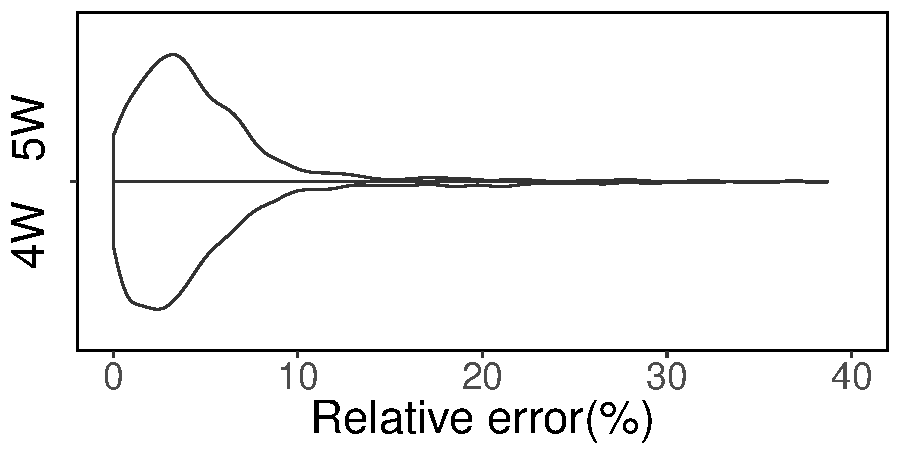
\includegraphics[height=15mm,width=30mm]{openmrs_linear_regression.pdf}}} & \multirow{1}[5]{*}{4W}    & \multirow{1}[5]{*}{23.24\%} & \multirow{2}[9]{*}{0.41} & \multicolumn{1}{c|}{\multirow{2}[9]{*}{N/A}} & \multirow{2}[4]{*}{{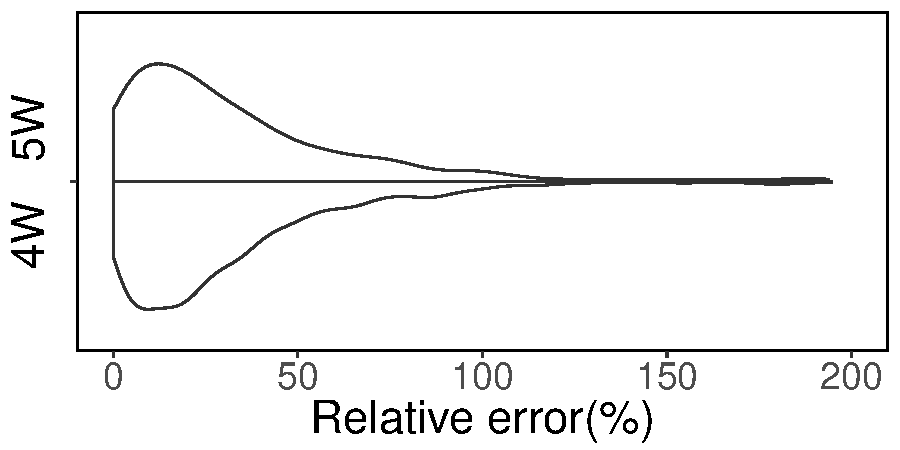
\includegraphics[height=15mm,width=30mm]{jms_linear_regression.pdf}}} \\[4.5mm]
\cline{2-3}\cline{7-8}          & \multirow{1}[5]{*}{5W}    & \multirow{1}[5]{*}{3.58\%} &       & (negligible) &       & \multirow{1}[5]{*}{5W}    & \multirow{1}[5]{*}{23.76\%} &       &       &  \\[4.5mm]
    \hline
    \multicolumn{1}{|c|}{\multirow{2}[9]{*}{Random 
Forest}} & \multirow{1}[5]{*}{4W}    & \multirow{1}[5]{*}{2.36\%} & \multirow{2}[9]{*}{\textless 0.01} & \multirow{1}[10]{*}{-0.09} & \multirow{2}[4]{*}{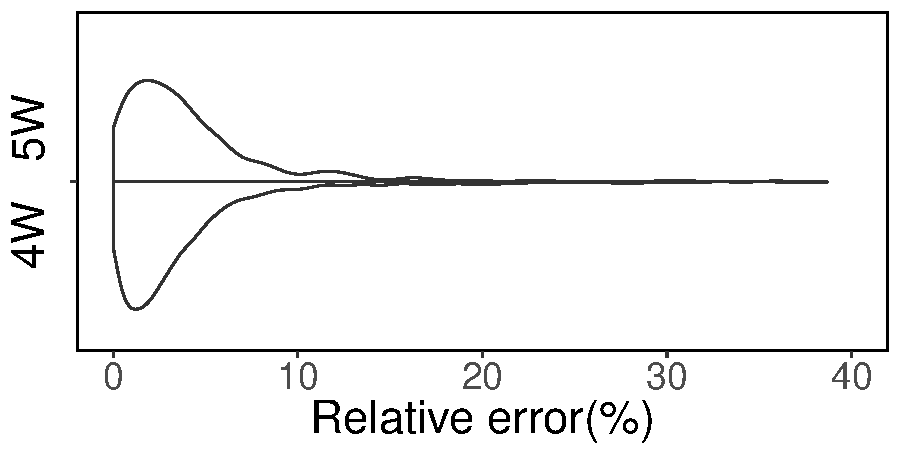
\includegraphics[height=15mm,width=30mm]{openmrs_random_forest.pdf}} & \multirow{1}[5]{*}{4W}    & \multirow{1}[5]{*}{22.99\%} & \multirow{2}[9]{*}{0.42} & \multicolumn{1}{c|}{\multirow{2}[9]{*}{N/A}} & \multirow{2}[4]{*}{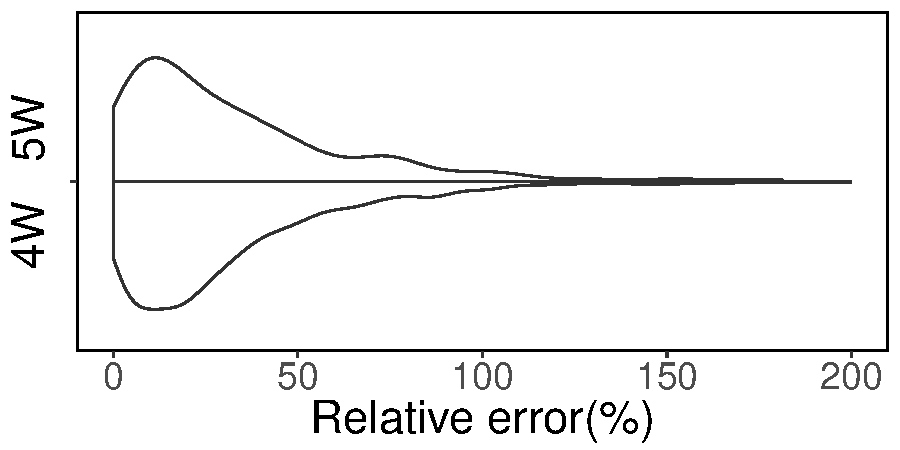
\includegraphics[height=15mm,width=30mm]{jms_random_forest.pdf}} \\[4.5mm]
\cline{2-3}\cline{7-8}          & \multirow{1}[5]{*}{5W}    & \multirow{1}[5]{*}{2.90\%} &       & (negligible) &       & \multirow{1}[5]{*}{5W}    & \multirow{1}[5]{*}{23.08\%} &       &       &  \\[4.5mm]
    \hline
    \multirow{2}[9]{*}{XGBoost} & \multirow{1}[5]{*}{4W}    & \multirow{1}[5]{*}{2.16\%} & \multirow{2}[9]{*}{0.14} & \multirow{2}[9]{*}{N/A} & \multirow{2}[4]{*}{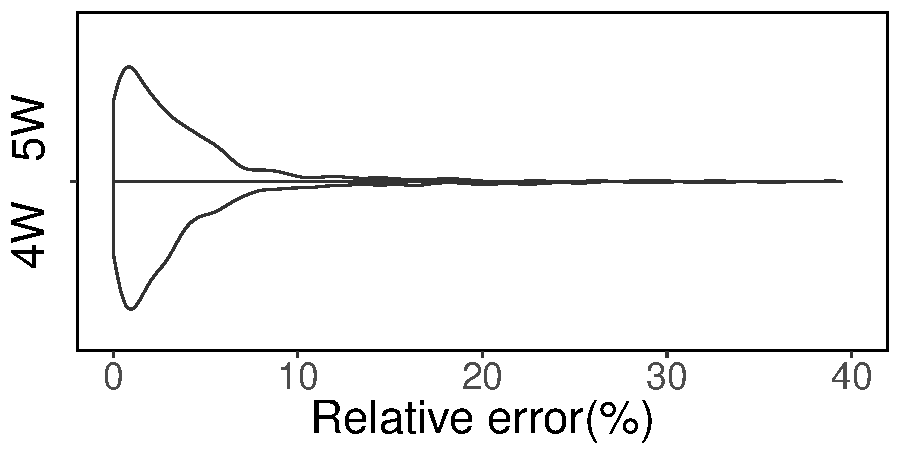
\includegraphics[height=15mm,width=30mm]{openmrs_xgboost.pdf}} & \multirow{1}[5]{*}{4W}    & \multirow{1}[5]{*}{24.29\%} & \multirow{2}[9]{*}{0.44} & \multirow{2}[9]{*}{N/A} & \multirow{2}[4]{*}{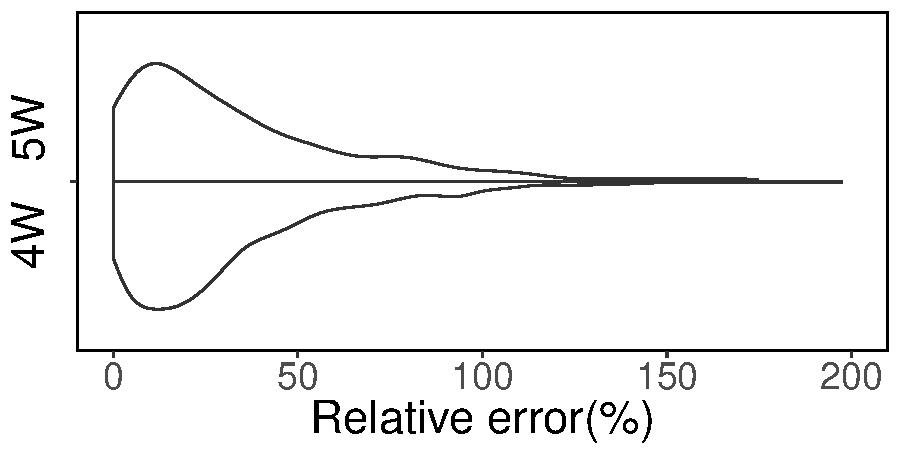
\includegraphics[height=15mm,width=30mm]{jms_xgboost.pdf}} \\[4.5mm]
\cline{2-3}\cline{7-8}          & \multirow{1}[5]{*}{5W}    & \multirow{1}[5]{*}{2.11\%} &       &       &       & \multirow{1}[5]{*}{5W}    & \multirow{1}[5]{*}{24.42\%} &       &       &  \\[4.5mm]
    \hline
    \multirow{2}[9]{*}{CNN} & \multirow{1}[5]{*}{4W}    & \multirow{1}[5]{*}{9.56\%} & \multirow{2}[9]{*}{\textless 0.01} & \multirow{1}[10]{*}{0.12} & \multirow{2}[4]{*}{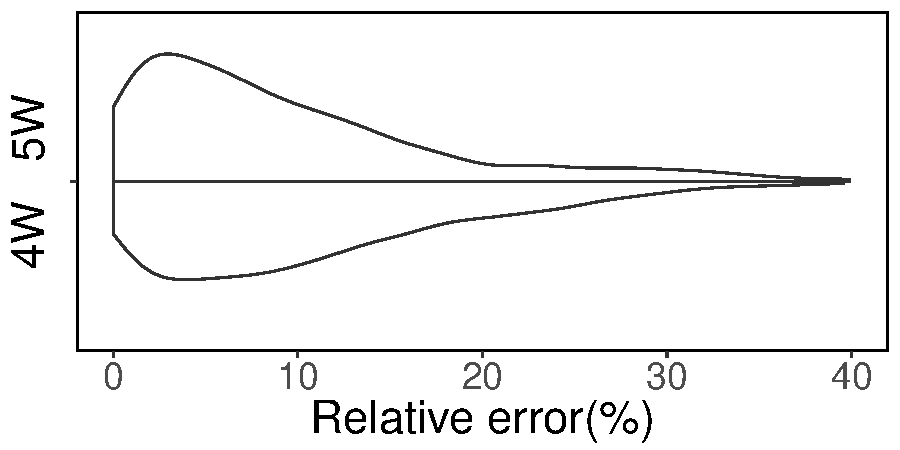
\includegraphics[height=15mm,width=30mm]{openmrs_cnn.pdf}} & \multirow{1}[5]{*}{4W}    & \multirow{1}[5]{*}{33.61\%} & \multirow{2}[9]{*}{0.11} & \multicolumn{1}{c|}{\multirow{2}[9]{*}{N/A}} & \multirow{2}[4]{*}{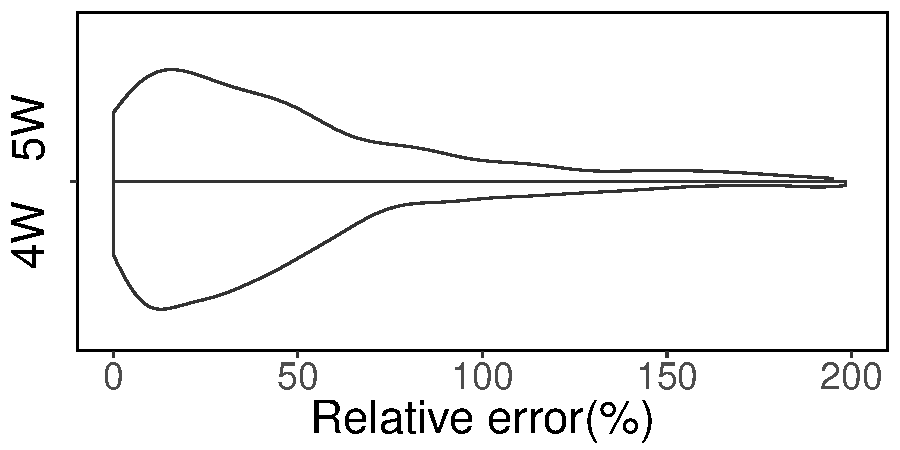
\includegraphics[height=15mm,width=30mm]{jms_cnn.pdf}} \\[4.5mm]
\cline{2-3}\cline{7-8}          & \multirow{1}[5]{*}{5W}    & \multirow{1}[5]{*}{7.47\%} &       & (negligible) &       & \multirow{1}[5]{*}{5W}    & \multirow{1}[5]{*}{37.51\%} &       &       &  \\[4.5mm]
    \hline
    \multirow{2}[9]{*}{RNN} & \multirow{1}[5]{*}{4W}    & \multirow{1}[5]{*}{5.63\%} & \multirow{2}[9]{*}{0.32} & \multirow{2}[9]{*}{N/A} & \multirow{2}[4]{*}{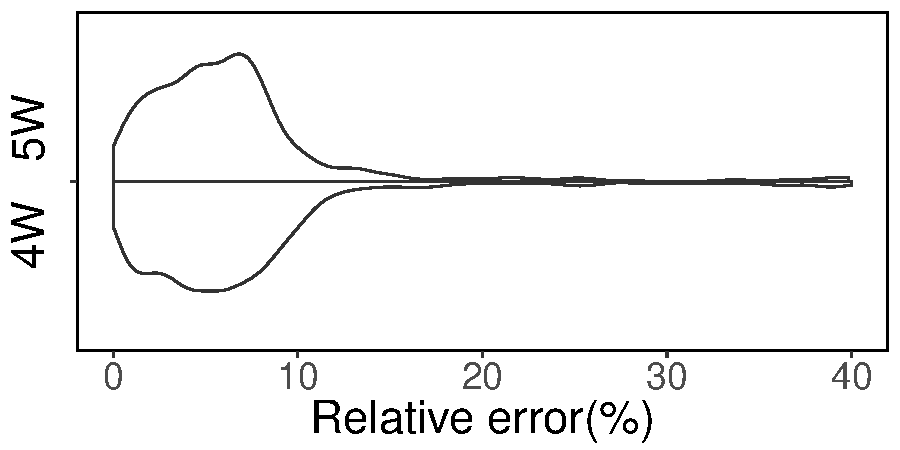
\includegraphics[height=15mm,width=30mm]{openmrs_rnn.pdf}} & \multirow{1}[5]{*}{4W}    & \multirow{1}[5]{*}{51.34\%} & \multirow{2}[9]{*}{0.01} & \multirow{1}[10]{*}{0.07} & \multirow{2}[4]{*}{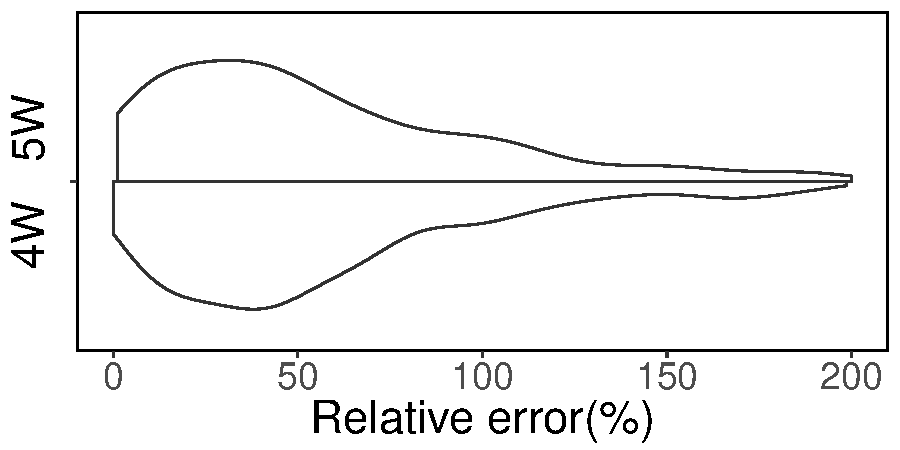
\includegraphics[height=15mm,width=30mm]{jms_rnn.pdf}} \\[4.5mm]
\cline{2-3}\cline{7-8}          & \multirow{1}[5]{*}{5W}    & \multirow{1}[5]{*}{5.73\%} &       &       &       & \multirow{1}[5]{*}{5W}    & \multirow{1}[5]{*}{47.22\%} &       & (negligible) &  \\[4.5mm]
    \hline
    \multirow{2}[9]{*}{LSTM} & \multirow{1}[5]{*}{4W}    &\multirow{1}[5]{*}{ 4.53\%} & \multirow{2}[9]{*}{\textless 0.01} & \multirow{1}[10]{*}{-0.25} & \multirow{2}[4]{*}{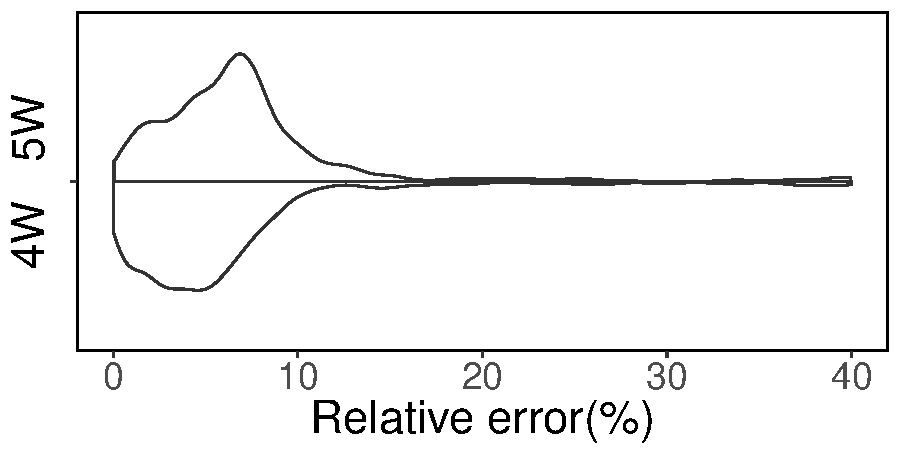
\includegraphics[height=15mm,width=30mm]{openmrs_lstm.pdf}} & \multirow{1}[5]{*}{4W}    & \multirow{1}[5]{*}{34.88\%} & \multirow{2}[9]{*}{\textless 0.01} & \multirow{1}[10]{*}{-0.27} & \multirow{2}[4]{*}{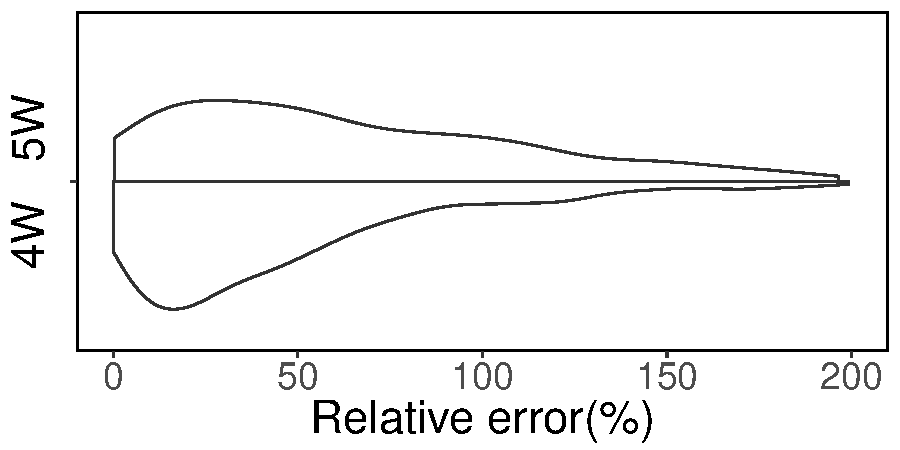
\includegraphics[height=15mm,width=30mm]{jms_lstm.pdf}} \\[4.5mm]
\cline{2-3}\cline{7-8}          & \multirow{1}[5]{*}{5W}    & \multirow{1}[5]{*}{6.42\%} &       & (small) &       & \multirow{1}[5]{*}{5W}    & \multirow{1}[5]{*}{57.11\%} &       & (small) &  \\[4.5mm]
    \hline
    \end{tabular}}
    Note: The column ``MRE'' presents the median relative errors.\hfill
  \label{tab:model_error}%
\end{table*}%
\end{landscape}

\noindent\textbf{Our black-box models can accurately model the performance of the studied systems using the dynamic runtime activities that are recorded in the logs.} 
As shown in Table \ref{tab:model_error}, the XGBoost model achieves the best results for modeling the performance of the OpenMRS system, with a median relative error of 2.11\% on the \emph{5W} workloads (i.e., the new workloads) and a median relative error of 2.16\% on the \emph{4W} workloads (i.e., the baseline workload). 
The random forest model achieves the best results for Apache James, reaching a median relative error of 22.99\% and 23.08\% for the \emph{4W} workloads and \emph{5W} workloads, respectively. 
All the machine learning models achieve better results for the OpenMRS system than the results for the Apache James system.
The less-promising results for the Apache James system might be explained by the latency between the actual activities of the mail server system and the recorded logs. For example, the system can take an extended period of time to process an email with a large attachment, while a log about the successful processing of the email is only printed after the processing period.

\noindent\textbf{The traditional models (e.g., linear regression and random forest) outperform the deep neural networks (e.g., CNN and RNN) for modeling the performance of the studied systems.}
As shown in Table~\ref{tab:model_error}, for both the OpenMRS and the Apache James systems, the three traditional models achieve better results than the three deep neural networks for modeling the system performance.
These results indicate that the relationship between the system performance and the runtime activities recorded in the logs can be effectively captured by the simple traditional models.
Such results also agree with a recent study~\citep{DacremaArxiv2019} that compares deep neural networks and traditional models for the application of automated recommendations.


\noindent\textbf{Our black-box models can equivalently explain the performance of a system under new workloads that are unseen when constructing the models.}
Table~\ref{tab:model_error} shows the statistical significance (i.e. the p-value) and the effect size of the difference between the prediction errors of applying the old models (i.e., trained from the \emph{4W} workloads) on the new workloads (i.e., the \emph{5W} workloads) and applying the old models on the old workloads (i.e., the \emph{4W} workloads). 
Table \ref{tab:model_error} also compares the distributions of the prediction errors for the \emph{4W} and \emph{5W} workloads.
The prediction errors of most of the models (except LSTM) have either statistically insignificant or negligible difference between the \emph{4W} and the \emph{5W} workloads, indicating that the models trained from the old workloads can equivalently model the system performance under new workloads.
The LSTM model results in a \emph{small} difference of the predictions errors between the \emph{4W} and the \emph{5W} workloads. We suspect that the complex LSTM model is likely over-fit towards the training workloads.

Due to an NDA, the detailed results of using the machine learning techniques to model the performance of the industry system (i.e, System X) are not presented in this paper. However, the results are similar to the shown results for the open source systems. In particular, when modeling the performance of all 10 studied versions of System X, the prediction errors are all between 10\% to 20\%. In addition, when we evaluate the models with different workloads, the differences between prediction errors are all either statistically insignificant or with negligible/small effect sizes.



\hypobox{Simple traditional models (e.g., linear regression and random forest) can accurately capture the relationship between the performance of a system and its dynamic activities that are recorded in logs, with varying workloads.
}

\subsection*{RQ2: Can our approach detect performance regressions under varying workloads?}

\subsubsection*{Motivation}

In traditional performance testing, in order to detect performance regressions, performance analysts compare the performance data of two versions of a software system that is generated by running the same workloads from the same performance test suites. 
However, in a field environment, as the workloads of the systems are constantly changing, it is almost impossible to run two software versions on the same workloads to detect performance regressions.
The results of RQ1 show that our black-box models can accurately capture the performance of a software system even under new workloads that are unseen when training the models.
Therefore, in this research question, we would like to leverage such black-box models to detect performance regressions when the workloads of the two versions of a system are not consistent.

Running the systems for hours or days before discovering performance regressions incurs a high cost. As the systems are already running in the field, any delay in detecting the performance regressions may pose huge impact on the end users. Hence, a desired approach in practice should be able to detect performance regression in a timely manner. Therefore, we also want to study how fast our approaches can detect performance regressions. 

\subsubsection*{Approach}

The results from RQ1 show that random forest and XGBoost have the lowest prediction errors when modeling performance (cf. Table~\ref{tab:model_error}). Since XGBoost requires resource-heavy fine-tuning, we opt to use random forest in this research question. For the open source systems, we first build the performance models from running the systems without performance regressions under the \emph{4W} workloads (i.e., a combination of four different concurrent workloads). We then run the systems without performance regressions under the \emph{5W} workloads (i.e., a combination of five different concurrent workloads). Ideally, our approach should not detect performance regressions from these runs. 
We use such results as a baseline to evaluate the effectiveness of our approach for detecting performance regressions under the new workloads (i.e., the \emph{5W} workloads). 
Afterwards, we run the systems with the performance regressions (cf. Table~\ref{tab:workloaddeisign}) under the \emph{5W} workloads. Our approach should be able to detect performance regressions from these runs.

For the System X from the industry, for every new release, we use our approach to compare the field data from the new release and the previous release to determine whether there are performance regressions. Since there are no injected or pre-known performance regressions, we present the detected performance deviance to the developers of the systems and manually study the code changes to understand whether the detection results are correct. For the releases that are detected as not having performance regressions, we cannot guarantee that these releases are free of performance regressions. However, we also present the results to the developers to confirm whether there exist any users who report performance-related issues for these releases. If so, our detection results may be considered false.

Finally, to study how fast our approaches can detect performance regressions, for the new versions of the systems that have performance regressions, we only use the first 15-minute data and apply our approach to detect the performance regressions. Then, we follow an iterative approach to add another 5-minute data to the existing data, until our approach can detect the performance regressions (i.e., with a medium or large effect size that is higher than the baseline). 

\subsubsection*{Results}

\noindent\textbf{Our black-box-based approaches can effectively detect performance regressions under varying workloads.}
Table~\ref{tab:predictionresult_rq2} shows the results of our three approaches of performance regression detection (cf. Section~\ref{sec:comparions-approaches}) on OpenMRS and Apache James. We find that with all three approaches, when there are known performance regressions between two versions, the statistical analysis always shows significant difference between the two versions with medium or large effect sizes. In addition, the effects sizes from Approach 1 and 2 are negative, confirming the existence of performance regressions (negative values indicate performance regression and positive values indicate performance improvement). 

When we compare the effect sizes with the baseline, i.e., running our approaches with systems without performance regressions but under two different workloads, we find that the baseline effect sizes are always smaller than the corresponding ones with performance regressions, except when detecting the regression in v3 of OpenMRS. We consider the reason being the nature of the regression in v3, i.e., an injected delay. Since our considered performance metric is the CPU usage and such a delay may not have large impact on the CPU usage, it is difficult for our approaches to detect such a regression. 


\begin{table}[tbh]
  \centering
  \tiny
  \tabcolsep=0.14cm
  \caption{Performance regression detection results for OpenMRS and Apache James. }
    \begin{tabular}{|c|c|c|c|c|c|c|c|}
    \hline
    \multicolumn{8}{|c|}{OpenMRS} \\
    \hline
    \multicolumn{2}{|c|}{Versions} & \multicolumn{2}{c|}{Approach 1} & \multicolumn{2}{c|}{Approach 2} & \multicolumn{2}{c|}{Approach 3} \\
    \hline
    \multicolumn{1}{|p{0.7cm}<{\centering}|}{Old\newline{}version} & \multicolumn{1}{|p{0.7cm}<{\centering}|}{New\newline{}version} & \multirow{1}[3]{*}{P-value} & \multirow{1}[3]{*}{Effect size} & \multirow{1}[3]{*}{P-value} & \multirow{1}[3]{*}{Effect size} & \multirow{1}[3]{*}{P-value} & \multirow{1}[3]{*}{Effect size} \\
    \hline
    v0 & v0 & $\ll$0.001 & 0.39 (medium) &  $\ll$0.001 & 0.36 (medium) & $\ll$0.001 & 0.17(small) \\
    \hline
    v0 & v1 & $\ll$0.001 & -0.59 (large) & $\ll$0.001 & -0.69 (large) & $\ll$0.001 & 0.38 (medium) \\
    \hline
    v0 & v2 & $\ll$0.001 & -0.44 (medium) & $\ll$0.001 & -0.63 (large) & $\ll$0.001 & 0.37 (medium) \\
    \hline
    v0 & v3 & $\ll$0.001 & -0.36 (medium) & $\ll$0.001 & -0.42 (medium) & $\ll$0.001 & 0.53 (large) \\
    \hline
    v0 & v4 & $\ll$0.001 & -0.69 (large) & $\ll$0.001 & -0.76 (large) & $\ll$0.001 & 0.51 (large) \\
    \hline
    \hline
    \multicolumn{8}{|c|}{Apache James} \\
    \hline
    \multicolumn{2}{|c|}{Versions} & \multicolumn{2}{c|}{Approach 1} & \multicolumn{2}{c|}{Approach 2} & \multicolumn{2}{c|}{Approach 3} \\
    \hline
    \multicolumn{1}{|p{0.7cm}<{\centering}|}{Old \newline{}version} & \multicolumn{1}{|p{0.7cm}<{\centering}|}{New \newline{}version} & \multirow{1}[3]{*}{P-value} & \multirow{1}[3]{*}{Effect size} & \multirow{1}[3]{*}{P-value} & \multirow{1}[3]{*}{Effect size} & \multirow{1}[3]{*}{P-value} & \multirow{1}[3]{*}{Effect size} \\
    \hline
    3.0m2 & 3.0m2 & 0.008 & 0.09 (negligible) & $\ll$0.001 & -0.12 (negligible) & $\ll$0.001 & -0.03 (negligible) \\
    \hline
    3.0m2 & 3.0m1 & $\ll$0.001 & -0.65 (large) & $\ll$0.001 & -0.76 (large) & $\ll$0.001 & 0.41 (medium) \\
    \hline
    3.0m2 & 2.3.2 & $\ll$0.001 & -0.90 (large) &$\ll$0.001 & -0.93 (large) & $\ll$0.001 & 0.82 (large) \\
    \hline
    \end{tabular}\\
    Note: For all the old versions, we use four concurrent workloads and for all the new versions with and without regressions, we use five concurrent workloads (one extra workload).\hfill
  \label{tab:predictionresult_rq2}%
\end{table}%

For all the 10 releases of System X, our approaches detected performance regressions from one release.
All three approaches detected performance regressions from the release with large effect sizes when compared with the previous release.
All three approaches did not detect performance regressions from the other nine releases (i.e., with either statistically insignificant difference or negligible effect sizes when compared with the previous release). 
By further investigating the release with performance regressions, we observed that developers added a synchronized operation to lock the resources that are responsible for generating a report, in order to protect the shared resources under the multi-thread situation. However, the reporting process is rather resource-heavy, resulting in significant overhead for each thread to wait and acquire the resources. Thus, the newly added lock causes the performance regression. After we discussed with the developers who are responsible for this module, we confirmed that this synchronized operation introduced performance regression to the software. 
In addition, for all the nine releases from which our approaches did not detect performance regressions, the developers of System X have not yet received any reported performance issues from the end users till the day of writing this paper.


\noindent\textbf{Comparing the prediction errors is more effective than comparing the prediction values when detecting performance regressions between two versions.}
We observe that for OpenMRS, the differences between the prediction values using Approach 1 and 2 can still be medium (0.39 and 0.36) even for the baseline (i.e., without regressions).
On the other hand, when comparing the prediction errors instead of the prediction values, i.e, using Approach 3, the baseline without regressions has only a small effect size (0.17).
Such a smaller baseline effect size makes Approach 3 easier to be adopted in practice, i.e., without the need of spending efforts searching for an optimal threshold on the effect size to detect performance regressions. However, Approach 3 only shows the deviance of the prediction errors without showing the direction of the performance deviance, thus it cannot distinguish a performance regression from a performance improvement. Hence, Approach 3 may be used first to flag the performance deviance then be combined with other approaches in practice to determine whether the performance deviation is a performance regression or a performance improvement.


\noindent\textbf{Our approaches can detect performance regressions as early as 15 minutes after running a new version.}
Table~\ref{tab:howearly} shows the earliest time that our approach can detect performance regressions in the studied open source systems. We find that all the performance regressions in the open source systems can be detected by at least one approach with less than 20-minute data from the new version. In particular, the regressions from both versions of Apache James and three versions of OpenMRS can even be detected using only the first 15-minute data. The ability of early detection eases the adoption of our approaches in the practices of testing in the field, where performance regressions are detected directly based on the field data, instead of using dedicated performance testing. 
 
\begin{table}[tbh]
  \centering
  \caption{The earliest time for our approaches to detect regressions in the two open source systems.}
    \begin{tabular}{c|cccc|cc}
    \hline
          & \multicolumn{4}{c|}{OpenMRS}  & \multicolumn{2}{c}{Apache James} \\
\cline{2-7}          & v1    & v2    & v3    & v4    & 3.0m1 & 2.3.2 \\
    \hline
    Approach 1 & 60 mins & 160 mins & 15 mins & 15 mins & 15 mins & 15 mins \\
    Approach 2 & 20 mins & 50 mins & 15 mins & 15 mins & 15 mins & 15 mins \\
    Approach 3 & 45 mins & 15 mins & 15 mins & 15 mins & 15 mins & 15 mins \\
    \hline
    \end{tabular}%
  \label{tab:howearly}%
\end{table}%



\hypobox{All three approaches can successfully detect performance regression under varying workloads, requiring data from a very short period of time (down to 15 minutes). 
Comparing the prediction errors is more effective than comparing the prediction values for detecting performance regressions between two versions.
}




\section{Challenges and Lessons Learned} \label{sec:challenges}
In this section, we discuss our faced challenges and learned lessons during applying our approach to the production environment of an industrial setting where a large number of customers worldwide access the system on a daily basis.

\newcounter{ChallengeCount}
\setcounter{ChallengeCount}{0}

\stepcounter{ChallengeCount}
\subsection*{C\arabic{ChallengeCount}: Determining the sampling frequency of performance metrics}
\noindent\textbf{Challenge.}
Our approach uses both logs and performance metrics as the input data to our black-box models. We use the logs that are automatically generated by the web servers, such as the Jetty, Tomcat, and IIS (Internet Information Services) web servers. 
The performance metrics (e.g., CPU, I/O) of the systems are collected using tools (e.g., \emph{Pidstat}).
A higher sampling frequency of the performance metrics can capture the system performance more accurately. However, a higher sampling frequency would also introduce more performance overhead. Since we need to apply our approach to the production environment, it is necessary to produce as low performance overhead as possible.

\noindent\textbf{Solution.}
At a first attempt, we intuitively chose 10 seconds as the sampling interval of the performance metrics. After we deployed our approach in production, we found that there is 0.5\%-0.8\% CPU overhead each time when our approach is collecting the performance metrics, and the overhead happens six times in 1 minute. Such a monitoring overhead cannot be ignored, especially when the system is serving heavy workloads. After working closely with the IT staffs from our industrial partner, we gained a deeper understanding of how the sampling frequency of performance metrics impact the monitoring overhead. Finally, we agreed that collecting the performance metrics for every 30 seconds would be a good balance between reducing the monitoring overhead and ensuring accuracy measurement of the system performance.

\noindent\textbf{Lessons learned.}
Monitoring a system usually comes with the monitoring overhead.
A higher monitoring frequency can provide a better monitoring accuracy at the cost of a larger monitoring overhead, which is usually undesirable when the system is serving large workloads.
Finding a good balance between the monitoring accuracy and the overhead is crucial for successful adoption of similar approaches in practice.


\stepcounter{ChallengeCount}
\subsection*{C\arabic{ChallengeCount}: Reducing the time cost of performance regression detection}
\noindent\textbf{Challenge.}
We choose random forest as our final black-box model to detect performance regressions, as random forest achieves the best results for modeling the performance of the studied systems (see RQ1).
A random forest model contains a configurable multitude of decision trees and takes the average output of the individual decision trees as the final output.
At first, we started with the default number of trees (i.e., 500 trees)~\citep{R-RandomForest}.
It took 5-6 hours to detect performance regressions between two releases of the industry system, including training and testing the random forest models and performing statistical tests. 
%\lizhi{it took 5-6 hours to training random forest models, predicting, and performing statistical analysis in order to detect performance regressions between two releases for the industry system, }
The industrial practitioners usually have an early need of checking if there is performance regression between the current version and multiple historical versions, which makes our approaches difficult to be adopted in a fast-paced development environment (e.g., an agile environment).

\noindent\textbf{Solution.}
A larger number of trees usually result in a more accurate random forest model, at the cost of longer training and prediction time.
In order to reduce the time cost of performance regression detection, we gradually decreased the number of trees in our random forest model while ensuring the model performance is not significantly impaired.
In the end, we kept 100 decision trees in our random forest models.
It took less than 2 hours to detect performance regressions between two releases of the industry system (i.e., training and testing the random forest models and performing statistical tests). 
% to detect performance regressions.
%\lizhi{building models, predicting, and yielding performance regressions detection results between two releases.}
Such a lighter model also enables us to detect performance regressions between the current version and multiple history versions (e.g., taking less than 10 hours when comparing the current version with five historical versions). 
We compared the prediction results of the 100-tree model with the original 500-tree models. We found that the 100-tree model only has a slightly higher median relative error (around 0.1\%) than the previous 500-tree models, which is negligible in practice.

\noindent\textbf{Lessons learned.}
In addition to the model performance, the time cost of training and applying a black-box model is also a major concern in the practice of performance regression detection in the field.
Seeking an appropriate trade-off between the model performance and the time cost is essential for the successful adoption of performance regression detection approaches in the field.


\stepcounter{ChallengeCount}
\subsection*{C\arabic{ChallengeCount}: Early detection of performance regressions}
\noindent\textbf{Challenge.}
In an in-house performance testing process, performance engineers usually wait until all the tests finish before they analyze the testing results.
However, in a field environment, any performance regressions can directly impact users' experience.
We cannot usually wait for a long time to gather plenty of data before performing performance analysis.
If our approach cannot detect performance regressions in a timely manner, the performance regressions would already have brought non-negligible negative impact to users.
This is a unique challenge facing the detection of performance regressions in the field.

\noindent\textbf{Solution.}
In order to detect field performance regressions in a timely manner, we continuously apply our approach to detect performance regressions using the currently available data.
For example, after a new version of the system has been up and running for one hour, we use only the one-hour data as our new workloads to determine the existence of performance regressions in the new versions.
Using the data generated in a short time period also allows the analysis part of our approach (i.e., model training and predictions) to be processed faster.
As discussed in RQ2, our approach can effectively detect performance regressions when the system has run for a very short time (e.g., down to 15 minutes for Apache James).
In other words, our approach can detect early performance regressions in the field.

\noindent\textbf{Lessons Learned.}
Different from performance regression detection in an in-house testing environment, performance regressions in the field need to be detected in a timely manner, in order to avoid notable performance impact to the users.
Continuously detecting performance regressions using the currently available data can help detect early performance regressions in the field.


\section{Threats to Validity} \label{sec:threats}

This section discusses the threats to the validity of our study.

\noindent \textbf{External validity.}
Our study is performed on two open source systems (i.e., OpenMRS and Apache James) and one industry system (i.e., System X) that are from different domains (e.g., health care system and mail server). 
All our studied systems are mature systems with years of history and have been studied in prior performance engineering research. Nevertheless, more case studies on other software systems in other domains can benefit the evaluation of our approach.
All our studied systems are developed in either Java or .Net. Our approach may not be directly applicable to systems developed in other programming languages, especially dynamic languages (e.g., JavaScript and Python). Future work may investigate approaches to minimize the uncertainty in the performance characterization of systems developed in dynamic languages.

\noindent \textbf{Internal validity.}
Our approach builds machine learning models to capture the relationship between the runtime activities that are recorded in logs and the measured performance of a system. 
However, there might be some runtime activities that are not recorded in logs and that also impact system performance.
In our approach, we use logs that capture the high-level workloads of the system. 
Our experiments on our studied systems demonstrated that such logs can predict system performance with a high accuracy.
Nevertheless, the correlation between the runtime activities recorded in the logs and the measured system performance does not necessarily suggest a causal relationship between them.


Our approach relies on non-parametric statistical analysis (i.e., Mann-Whitney U test and Cliff's delta) to compare the black-box behaviors of two software versions to detect performance regressions. 
Our assumption is that statistically different behaviors between two software versions would suggest performance regressions.
In practice, however, determining whether there is a performance regression usually depends on the subjective judgement of the performance analysts.
Therefore, our approach enables performance analysts to adjust the threshold of the statistics (e.g., the effect size) to detect performance regressions in their specific scenarios.

\noindent \textbf{Construct validity.}
In this work, we use the CPU usage as our performance metric to detect performance regressions.
There exist other performance metrics, such as memory utilization and response time that can be considered to detect performance regressions. 
Considering other performance metrics would benefit our approach.
However, monitoring more performance metrics would introduce more performance overhead to the monitored system.
In the case of our industry system, the CPU usage is the main concern in performance regression detection.
Besides, the three studied approaches are not limited to the performance metric of CPU usage. Practitioners can leverage our approach to consider other performance metrics that are appropriate in their context.

\section{Related Work}
\label{sec:relatedwork}

In this section, we discuss prior work along three dimensions: software performance regression detection, performance model for configurable system, and identifying optimal configuration for performance. % engineering.

\subsection{Performance regression detection}
Extensive prior research has proposed automated techniques to detect performance regressions. Such detection techniques can be divided into two categories: measurement-based and model-based detection. 

Measurement-based approaches compare performance metrics (e.g., CPU usage) between two consecutive versions to detect performance regressions. %measure performance metrics and compares these performance metrics between two consecutive versions of a system to detect performance regression. 
For example, Nguyen \emph{et al$.$}~\cite{Nguyen:2012:ADP,nguyen2011automated,Nguyen:2014:ICS} %conducted a series of studies on performance regressions. Nguyen \emph{et al$.$} apply control charts to analyze performance counters across test runs to detect performance regression automatically. They construct the control chart to detect performance regressions  by setting upper and lower bounds of performance counters.
leveraged control charts to identify performance regressions. %~\heng{treat regression as a countable word throughout the paper, countable seems better}. 
A control chart has an upper control limit and a lower control limit. A performance regression is detected when a performance metric is above the upper limit or below the lower limit. Foo \emph{et al$.$}~\cite{foo2010mining} proposed an approach that compares a test's performance metrics to historical performance metrics. %\med{from what?}performance regression testing repositories to detect potential performance regressions. 

A model-based approach builds %\med{This paragraph is difficult to understand. What is detected model? is it prediction model? and what is counters? what is signatures? what do you mean by heterogeneous environment?} 
%\jinfu{detected model is a general model, we can use model. Performance counter is performance metric, like CPU usage. Some papers use signatures to represent system users' behavior.} \med{I updated this paragraph, though Bodik work is not clear} 
a machine learning model with a set of performance metrics to detect performance regressions.  Cohen et al.~\cite{Cohen:2005:CIC} showed an implication that it is ineffective and not enough to index and identify performance problems with simple records of raw system metrics. Cohen et al. used TAN (Tree-Augmented Bayesian Network) models to model the system performance states based on a small subset of metrics. %Therefore, the authors present an approach to capture signatures representing system states from a running system and cluster such signitures to detect recurrent or similar performance problems. 
Bodik \emph{et al$.$}~\cite{bodik2008hilighter} leveraged a logistic regression model to model system users' behavior to improve Cohen \emph{et al$.$}\textquotesingle s model. %~\heng{need to mention Cohen's model beforehand}. 
Foo \emph{et al$.$}~\cite{DBLP:conf/icse/FooJAHZF15} proposed an approach that uses ensembles of models to detect performance regressions in heterogeneous environments (e.g., different hardware and software configurations). % \med{examples of what heterogeneous environments} \jinfu{different hardware and software configurations}). 
Xiong \emph{et al$.$}~\cite{Xiong:2013:VAM} proposed a model-driven framework to diagnose application performance and identify the root cause of performance issues. %Such framework uses linear regression to build the predict model to automatically diagnose the system performance in cloud environment and lead to root cause of performance problem.

%\med{well, we predict it, so it's kind of detecting performance regression}Our research is not designed to detect performance regression. The goal of our research is to examine the impact of configuration options on the performance regression. In our paper, we conduct measurement-based approach to identify performance regression on the commit level.

%\med{is the following paragraph correct?}
Our work complements this line of research in the sense that we consider the configuration aspect of highly configurable software systems. For instance, a code change might not show a performance regression on the default configuration, while leading to regressions on other configurations. This paper sheds light on the \inconsistent problem by first quantifying the existence of inconsistent performance variations, then proposing a prediction model that identifies the commits, tests, and options that exhibit the \inconsistent problem. 


\subsection{Performance model for configurable system}
Many prior research has been conducted on predicting performance for configurable software systems. 
M{\"{u}}hlbauer et al.~\cite{DBLP:conf/kbse/MuhlbauerAS19,DBLP:conf/kbse/MuhlbauerAS20} build performance model to identify performance changes in software performance evolution. The authors combine active learning and Gaussian process regression to model and estimate a software system’s performance evolution with only performance measurements based on a few revisions. Such prior study provides an evidence that performance changes during software evolution, which motivates our study. Jamshidi et al.~\cite{DBLP:conf/kbse/JamshidiSVKPA17,DBLP:conf/icse/JamshidiVKSK17,DBLP:conf/sigsoft/JamshidiVKS18} employ transfer learning to learn performance model across environments. Work~\cite{DBLP:conf/kbse/JamshidiSVKPA17} conducts an exploratory study on four systems to investigate how a performance model for a configurable system changes when the system is deployed in different environments. The result shows that for severe environmental changes, a considerable part of invalid configuration is preserved across environmental changes. Following the exploratory study, Jamshidi et al.~\cite{DBLP:conf/icse/JamshidiVKSK17} propose an approach to learn the performance model for a real system using other sources such as simulator with a few measurements at a lower cost. The results show that transfer learning can achieve high prediction accuracy with only a few samples from the real-world system. Jamshidi et al.~\cite{DBLP:conf/sigsoft/JamshidiVKS18} propose learning to sample (L2S) that extract transferable knowledge from the source environment to help sample the configurations in the target environment. DeepPerf~\cite{DBLP:conf/icse/HaZ19} uses a deep feed-forward neural network to model configurable software system. Results show that DeepPerf can predict a system's performance with a small sample of configuration. 

The existing studies use the historical revisions’ performance, or the sampled configuration’s performance to build a model, to estimate the performance of future revisions. Different from prior studies, we consider all the configuration options and collect real performance data. In addition, we aim to find the inconsistent option performance variations during software evolution. In general, our study is orthogonal to the above approaches and our measured performance data can be used in future research on performance.

\subsection{Identifying optimal configuration for performance} 
A large body of research has been conducted on performance optimization by finding optimal configuration. 
Siegmund et al.~\cite{RN2880} build mathematical models that describe the impact of a configuration on software performance based on each option's value. Raghavachari et al.~\cite{RN3537} propose an iterative approach to identify an optimal configuration in terms of performance. Their approach consists of selecting for a J2EE web application a first configuration, compare its performance to a second configuration until the optimal configuration is found. Similarly, Dia et al.~\cite{RN3543} propose an approach that automatically adjusts the values of existing configuration options at run-time to optimize the CPU and memory usage objectives.
Li et al.~\cite{LiAutoConfig} leveraged performance monitoring data and execution logs to dynamically optimize the values of performance-related configuration options according to varying workloads in the field. 
Guo et al.~\cite{RN3544} leverage non-linear regression to suggest an optimal configuration.
It was extended to DECART~\cite{DBLP:journals/ese/GuoYSASVCWY18} that combines the CART with automated resampling and parameter tuning to predict performance of configurable systems. However, collecting a large amount of data for training a model that predicts the performance of a configuration is expensive.
Therefore, Sarkar et al.~\cite{RN3089} evaluated the progressive and projective sampling to train a model that predicts the performance of configuration. For their initial training sample, they consider data on which each option is enabled at least once. 
Nair et al.~\cite{DBLP:conf/sigsoft/NairMSA17,DBLP:journals/tse/Nair0MSA20} conduct several studies to find well-performing configurations. 
Nair et al.~\cite{DBLP:conf/sigsoft/NairMSA17} first propose a rank-based approach that uses the performance model building from a few sample configurations, to rank the configurations, in order to find the faster configurations. 
Nair et al.~\cite{DBLP:journals/tse/Nair0MSA20} also propose a novel approach named FLASH that use a sequential model-based approach to find better configurations for a software system. 
Oh et al.~\cite{DBLP:conf/sigsoft/OhBMS17} propose a truly random sampling to search configurations recursively to find near-optimal configurations without building a performance model.
Other efforts identified the optimal configuration options in terms of performance by leveraging existing optimization approaches, i.e., iterative search~\cite{RN3545}, multi-objective optimization~\cite{singh2016optimizing}, and smart hill climbing~\cite{RN3518}.

This paper’s goal is neither to identify optimal configurations nor to debug configuration-related performance issues. Instead, we focus on studying inconsistent option performance through different commits. In particular, we focus on understanding whether a performance improvement or regression is consistent through all the values of an option. That is important, as one can improve the performance of a software system or release new changes that do not impact the performance under one configuration when other configurations hide a performance regression. 
Furthermore, prior work on this line of research compares the absolute performance between two values for the same option, while this can be subjective, as discussed earlier. One option's value can naturally consume performance as it enables the execution of additional features. However, performance comparison need also consider historical performance data. For instance, the execution of the software system under the same option's value can be improved %\bram{for those features? flow in this paragraph is unclear} 
compared the same option and value prior to that commit. In addition, a better performing option's value can show a regression compared to the prior commit as well. %impact of configuration options on the performance regression.% While a new commit does not show any performance regression under the default configuration, other configurations might show a low performance when the same configuration showed a good performance in the prior commit. 

%\subsection{Software Configuration}

%A large body of research efforts have been conducted on software configuration, which mainly focus on understanding configuration problems, preventing configuration errors, and debugging configuration errors. In this Section, we focus on the efforts that are related to the performance of configuration, while we refer to our prior systematic literature review~\cite{tse} for more details. %Few research efforts consider the performance aspect of software configuration \bram{wasn't there a lot of work on performance tuning in Mohammed's TSE survey?}. 

%\subsubsection{Understanding Configuration Problems}
%Configuration makes a software system complex~\cite{tse}, which leads to configuration errors that are severe, common, and hard to debug~\cite{RN3251}. For instance, Jin et al.~\cite{RN2897} found that configuration options add more complexity to the development and testing of highly configurable software systems. Han et al.~\cite{RN2864} found that configuration options are responsible for 59\% of the performance bugs. Gousios et al.~\cite{RN3551} observed that the configuration of the garbage collectors have an impact on the performance of server applications. Furthermore, Sayagh et al.~\cite{RN3249, RN2758} found that the impact of a configuration option can spread to multiple layers of an architectural stack.% Jin et al.~\cite{RN2897} found that there is a need for tools that debug configuration errors in multi-languages software systems. 

%Our work is different from this line of research as we consider the performance regression that is caused by configuration options.
%\subsubsection{Debugging Configuration Errors} 
%A second line of research proposed and evaluated different approaches to identify misconfigured configuration options. Dong et al.\cite{RN2805, RN3163} leverage the slicing technique to identify the misconfigured option for a given error message or exception. Rabkin et al.~\cite{RN2822} leverage a data flow analysis technique to identify for each option, which source code lines it might impacts. Attaryian et al.~\cite{RN3248} combined dynamic control and data flow analysis to identify misconfigured options. Zhang et al.~\cite{RN2839, RN2777} compared the trace of a correct execution against the trace of an incorrect execution to identify culprit options. We refer to our prior systematic literature review~\cite{tse} and the work of Tianyin et al.~\cite{RN3252} and Andrzejak et al.\cite{andrzejaksoftware} for further details about the existing configuration debugging approaches. 

%Our work is different from this line of research since we do not consider debugging configuration errors, but understanding and identifying performance regressions that are caused under certain configurations.

%\subsubsection{The Performance of Configurations} 

\begin{comment}
\subsection{Configuration-related performance bug}
Another line of research considers the debugging of performance errors that are caused by configuration options.
Attariyan et al.~\cite{RN3253} proposed an approach based on dynamic taint analysis technique to identify the option that causes a performance error. % assigns to each source code block a cost, use a dynamic analysis techniques that instruments and runs a software system, then their approach identifies which blocks were executed and which options they depends on. 
\end{comment}

\begin{comment}
Another line of research considers the identification of the optimal configurations for a software system and the debugging of performance errors that are caused by configuration options. 


Attariyan et al.~\cite{RN3253} proposed an approach based on dynamic taint analysis technique to identify the option that causes a performance error. % assigns to each source code block a cost, use a dynamic analysis techniques that instruments and runs a software system, then their approach identifies which blocks were executed and which options they depends on. 
Siegmund et al.~\cite{RN2880} build mathematical models that describe the impact of a configuration on software performance based on each option's value. Raghavachari et al.~\cite{RN3537} propose an iterative approach to identify an optimal configuration in terms of performance. Their approach consists of selecting for a J2EE web application a first configuration, compare its performance to a second configuration until the optimal configuration is found. Similarly, Dia et al.~\cite{RN3543} propose an approach that automatically adjusts the values of existing configuration options at run-time to optimize the CPU and memory usage objectives.

Li et al.~\cite{LiAutoConfig} leveraged performance monitoring data and execution logs to dynamically optimize the values of performance-related configuration options according to varying workloads in the field. Guo et al.~\cite{RN3544} leverage non-linear regression to suggest an optimal configuration. However, collecting a large amount of data for training a model that predicts the performance of a configuration is expensive. Therefore, Sarkar et al.~\cite{RN3089} evaluated the progressive and projective sampling to train a model that predicts the performance of configuration. For their initial training sample, they consider data on which each option is enabled at least once. Other efforts identified the optimal configuration options in terms of performance by leveraging existing optimization approaches, i.e., iterative search~\cite{RN3545}, multi-objective optimization~\cite{singh2016optimizing}, and smart hill climbing~\cite{RN3518}.
\end{comment}



\begin{comment}

\subsection{Software Performance}

Performance is an important aspect of software quality. Extensive prior research has been conducted to study software performance. In this subsection, we summarize the empirical studies on  %performance to 
understanding software performance and the studies on %. We then present the related works of 
performance regression detection.

\subsubsection{Empirical Studies on Software Performance}
Several empirical studies have been conducted on the performance of software systems~\cite{ICSE2014:Huang,Jin:2012,MSR11:Zaman,MSR12:Zaman,DBLP:conf/kbse/HanYL18,Leitner2017ICPE}. For instance, Jin \emph{et al$.$}~\cite{Jin:2012} studied 109 real-world performance issues that are reported from five open source software systems and %. Based on the studied 109 performance bugs, the authors 
%developed an automated tool 
proposed an approach to detect performance issues. Zaman \emph{et al$.$}~\cite{MSR11:Zaman,MSR12:Zaman} conducted qualitative and quantitative studies on performance issues. They found that developers and users face problems in reproducing performance bugs %. More time is 
as they spend % 
a lot of time discussing performance bugs %than 
compared to other kinds of bugs (e.g., functional bugs). %\jinfu{For example, Firefox performance bugs take more time to discuss and fix.\med{I meant examples of other kinds of bugs}} 
Huang \emph{et al$.$}~\cite{ICSE2014:Huang} %studied real world performance issues. They 
proposed an approach to improve the efficiency of performance regression testing by leveraging a static analysis technique to estimate the risk of a given commit in introducing a performance regression. Han et al$.$~\cite{DBLP:conf/kbse/HanYL18} studied %y
300 bug reports from three large open source projects. The authors found that most of the performance bugs occur for specific combinations of data input and configurations. They also proposed a framework named \emph{PerfLearning} to extract such data input and configurations from bug reports to generate test frames. Leitner et al$.$~\cite{Leitner2017ICPE} %aim to understand the current state of art of performance testing. They conduct a study on 111 open-source java-based systems from GitHub 
investigated the state-of-the-practice related to performance tests. The authors found that performance tests form only a small portion of a test suite.
%and use a combination of quantitative and qualitative research methods to investigate the use of performance tests across five perspectives.

The vast amount of research on software performance signifies its importance and motivates our work. %Prior studies on performance typically are based on either limited performance issue reports or release of the software. 
Different from prior research, we evaluate software performance at the commit level and study performance regressions that are manifested under a subset of the possible configurations. % by configuration option.
In addition, our work is different from this line of research as we consider how to avoid performance regressions that are related to some configurations while being hidden by other configurations, instead of understanding the existing performance related issues. 

\subsubsection{Performance regression detection}
Extensive prior research has proposed automated techniques to detect performance regressions. Such detection techniques can be divided into two categories: measurement-based and model-based detection. 

Measurement-based approaches compare performance metrics (e.g., CPU usage) between two consecutive versions to detect performance regressions. %measure performance metrics and compares these performance metrics between two consecutive versions of a system to detect performance regression. 
For example, Nguyen \emph{et al$.$}~\cite{Nguyen:2012:ADP,nguyen2011automated,Nguyen:2014:ICS} %conducted a series of studies on performance regressions. Nguyen \emph{et al$.$} apply control charts to analyze performance counters across test runs to detect performance regression automatically. They construct the control chart to detect performance regressions  by setting upper and lower bounds of performance counters.
leveraged control charts to identify performance regressions. %~\heng{treat regression as a countable word throughout the paper, countable seems better}. 
A control chart has an upper control limit and a lower control limit. A performance regression is detected when a performance metric is above the upper limit or below the lower limit. Foo \emph{et al$.$}~\cite{foo2010mining} proposed an approach that compares a test's performance metrics to historical performance metrics. %\med{from what?}performance regression testing repositories to detect potential performance regressions. 

A model-based approach builds %\med{This paragraph is difficult to understand. What is detected model? is it prediction model? and what is counters? what is signatures? what do you mean by heterogeneous environment?} 
%\jinfu{detected model is a general model, we can use model. Performance counter is performance metric, like CPU usage. Some papers use signatures to represent system users' behavior.} \med{I updated this paragraph, though Bodik work is not clear} 
a machine learning model with a set of performance metrics to detect performance regressions.  Cohen et al.~\cite{Cohen:2005:CIC} showed an implication that it is ineffective and not enough to index and identify performance problems with simple records of raw system metrics. Cohen et al. used TAN (Tree-Augmented Bayesian Network) models to model the system performance states based on a small subset of metrics. %Therefore, the authors present an approach to capture signatures representing system states from a running system and cluster such signitures to detect recurrent or similar performance problems. 
Bodik \emph{et al$.$}~\cite{bodik2008hilighter} leveraged a logistic regression model to model system users' behavior to improve Cohen \emph{et al$.$}\textquotesingle s model. %~\heng{need to mention Cohen's model beforehand}. 
Foo \emph{et al$.$}~\cite{DBLP:conf/icse/FooJAHZF15} proposed an approach that uses ensembles of models to detect performance regressions in heterogeneous environments (e.g., different hardware and software configurations). % \med{examples of what heterogeneous environments} \jinfu{different hardware and software configurations}). 
Xiong \emph{et al$.$}~\cite{Xiong:2013:VAM} proposed a model-driven framework to diagnose application performance and identify the root cause of performance issues. %Such framework uses linear regression to build the predict model to automatically diagnose the system performance in cloud environment and lead to root cause of performance problem.

%\med{well, we predict it, so it's kind of detecting performance regression}Our research is not designed to detect performance regression. The goal of our research is to examine the impact of configuration options on the performance regression. In our paper, we conduct measurement-based approach to identify performance regression on the commit level.

%\med{is the following paragraph correct?}
Our work complements this line of research in the sense that we consider the configuration aspect of highly configurable software systems. For instance, a code change might not show a performance regression on the default configuration, while leading to regressions on other configurations. This paper sheds light on the \inconsistent problem by first quantifying the existence of inconsistent performance variations, then proposing a prediction model that identifies the commits, tests, and options that exhibit the \inconsistent problem. 

\end{comment} 

\section{Conclusions} \label{sec:conclusions}

%Performance regressions in large-scale software systems usually leads to reputational and monetary losses.
%Traditionally, practitioners perform in-house performance testing to detect such performance regressions.
%However, such in-house performance testing is usually very expensive and difficult to simulate the constantly-changing workloads from the field.

In this paper, we propose to leverage automated approaches   %, \emph{FRDetector}, 
that can effectively detect early performance regressions in the field. 
We study three approaches that use black-box performance models to capture the relationship between the activities of a software system and its performance under such activities, and then compare the black-box models derived from the current version of a software system and an earlier version of the same software system, to determine the existence of performance regressions between these two versions.
By an empirical study on two open source systems (OpenMRS and Apache James) and one large-scale industry system, we found that simple black-box models (e.g., random forest) can accurately capture the relationship between the performance of a system under varying workloads and its dynamic activities that are recorded in logs.
%Besides, such models can equivalently explain the performance of a system under new workloads unseen when building the models.
We also found that these black-box models can effectively detect real performance regressions and injected performance regressions under varying workloads, requiring data from only a short period of operations.
Our approaches can complement or even replace typical in-house performance testing when testing resources are limited (e.g., in an agile environment).
The challenges and the lessons that we learned from the successful adoption of our approach also provide insights for practitioners who are interested in performance regression detection in the field.

\section*{Acknowledgement}
We would like to thank ERA Environmental Management Solutions
for providing access to the enterprise system used in our case study.
The findings and opinions expressed in this paper are those of the
authors and do not necessarily represent or reflect those of ERA
Environmental Management Solutions and/or its subsidiaries and
affiliates. Moreover, our results do not reflect the quality of ERA
Environmental Management Solutions’ products.

%Import the natbib package and sets a bibliography  and citation styles
\bibliographystyle{natbib}

\bibliography{detectregression}


% that's all folks
\end{document}


